%%%%%%%%%%%%%%%%%%%%%%%%%%%%%%%%%%%%%%%%%%%%%%%%%%%%%%%%%%%%%%%%%%%%%%%%%%%%%%%%
%% Plantilla de memoria en LaTeX para la ETSIT - Universidad Rey Juan Carlos
%%
%% Por Gregorio Robles <grex arroba gsyc.urjc.es>
%%     Grupo de Sistemas y Comunicaciones
%%     Escuela Técnica Superior de Ingenieros de Telecomunicación
%%     Universidad Rey Juan Carlos
%% (muchas ideas tomadas de Internet, colegas del GSyC, antiguos alumnos...
%%  etc. Muchas gracias a todos)
%%
%% La última versión de esta plantilla está siempre disponible en:
%%     https://github.com/gregoriorobles/plantilla-memoria
%%
%% Para obtener PDF, ejecuta en la shell:
%%   make
%% (las imágenes deben ir en PNG o JPG)

%%%%%%%%%%%%%%%%%%%%%%%%%%%%%%%%%%%%%%%%%%%%%%%%%%%%%%%%%%%%%%%%%%%%%%%%%%%%%%%%

\documentclass[a4paper, 12pt, english]{book}
\usepackage[T1]{fontenc}


\usepackage[a4paper, left=2.5cm, right=2.5cm, top=3cm, bottom=3cm]{geometry}
\usepackage{times}
%\usepackage[spanish]{babel} % Comenta esta línea si tu memoria es en inglés
\usepackage{url}
%\usepackage[dvipdfm]{graphicx}
\usepackage{graphicx}
\usepackage{float}  %% H para posicionar figuras
\usepackage[nottoc, notlot, notlof, notindex]{tocbibind} %% Opciones de índice
\usepackage{latexsym}  %% Logo LaTeX

\usepackage[T1]{fontenc}
\usepackage{selinput}
\SelectInputMappings{%
  aacute={á},
  ntilde={ñ},
  Euro={€}
}
\usepackage{babel}

\usepackage{hyperref}

\usepackage{listings}
\usepackage{color}
\usepackage{titlesec}
\usepackage{epigraph}

\titleclass{\subsubsubsection}{straight}[\subsection]

\newcounter{subsubsubsection}[subsubsection]
\renewcommand\thesubsubsubsection{\thesubsubsection.\arabic{subsubsubsection}}
\renewcommand\theparagraph{\thesubsubsubsection.\arabic{paragraph}} % optional; useful if paragraphs are to be numbered

\titleformat{\subsubsubsection}
  {\normalfont\normalsize\bfseries}{\thesubsubsubsection}{1em}{}
\titlespacing*{\subsubsubsection}
{0pt}{3.25ex plus 1ex minus .2ex}{1.5ex plus .2ex}

\makeatletter
\renewcommand\paragraph{\@startsection{paragraph}{5}{\z@}%
  {3.25ex \@plus1ex \@minus.2ex}%
  {-1em}%
  {\normalfont\normalsize\bfseries}}
\renewcommand\subparagraph{\@startsection{subparagraph}{6}{\parindent}%
  {3.25ex \@plus1ex \@minus .2ex}%
  {-1em}%
  {\normalfont\normalsize\bfseries}}
\def\toclevel@subsubsubsection{4}
\def\toclevel@paragraph{5}
\def\toclevel@paragraph{6}
\def\l@subsubsubsection{\@dottedtocline{4}{7em}{4em}}
\def\l@paragraph{\@dottedtocline{5}{10em}{5em}}
\def\l@subparagraph{\@dottedtocline{6}{14em}{6em}}
\makeatother

\setcounter{secnumdepth}{4}
\setcounter{tocdepth}{4}


\definecolor{nd}{RGB}{98, 143, 217}
\definecolor{keyword}{RGB}{255,51,102}
\definecolor{bg}{RGB}{255, 255, 232}
\definecolor{comment}{RGB}{73, 79, 92}
\definecolor{str}{RGB}{30, 184, 135}

\lstdefinelanguage{Sass}{
	keywords={mixin, keyframe, include, import, extend, class, \@},
	keywordstyle=\color{keyword},
	indentifierstyle=\color{black}\bfseries,
	sensitive=false,
	comment=[l]{\#},
  	morecomment=[s]{/*}{*/},
    	commentstyle=\color{comment}\ttfamily
}

\lstdefinelanguage{JavaScript}{
 	keywords={\$, const, constructor, typeof, new, true, false, catch, function, return, null, catch, switch, var, if, in, while, do, else, case, break},
  	keywordstyle=\color{keyword},
  	ndkeywords={private, public, Router, class, export, boolean, Number, throw, implements, import, this, prototype, then, string, any},
  	ndkeywordstyle=\color{nd}\bfseries,
  	identifierstyle=\color{black},
  	sensitive=false,
  	comment=[l]{//},
  	morecomment=[s]{/*}{*/},
  	commentstyle=\color{comment}\ttfamily,
  	stringstyle=\color{str}\ttfamily,
  	morestring=[b]',
  	morestring=[b]"
}

\lstset{
frame=single,
   language=Javascript,
   backgroundcolor=\color{bg},
   extendedchars=true,
   basicstyle=\small\ttfamily,
   showstringspaces=false,
   showspaces=false,
   numbers=left,
   numberstyle=\footnotesize,
   numbersep=9pt,
   tabsize=2,
   breaklines=true,
   showtabs=false,
   captionpos=b,
   xleftmargin=\parindent,
}

\title{Memoria del Proyecto}
\author{Ismael Slimane Zubillaga}

\renewcommand{\baselinestretch}{1.5}  %% Interlineado
\Urlmuskip=0mu plus 2mu

\begin{document}

\renewcommand{\refname}{Bibliografía}  %% Renombrando
\renewcommand{\appendixname}{Apéndice}

%%%%%%%%%%%%%%%%%%%%%%%%%%%%%%%%%%%%%%%%%%%%%%%%%%%%%%%%%%%%%%%%%%%%%%%%%%%%%%%%
% PORTADA

\begin{titlepage}
\begin{center}
\begin{tabular}[c]{c c}
%\includegraphics[bb=0 0 194 352, scale=0.25]{logo} &

\includegraphics[scale=0.25]{img/logo_vect.png} &
\begin{tabular}[b]{l}
\Huge
\textsf{UNIVERSIDAD} \\
\Huge
\textsf{REY JUAN CARLOS} \\
\end{tabular}
\\
\end{tabular}

\vspace{3cm}

\Large
INGENIERÍA EN TECNOLOGÍAS DE LA TELECOMUNICACIÓN

\vspace{0.4cm}

\large
Curso Académico 2017/2018

\vspace{0.8cm}

Trabajo Fin de Grado/Máster

\vspace{2.5cm}

\LARGE
ANGULAR-BASED DASHBOARD FOR ELASTICSEARCH

\vspace{4cm}

\large
Autor : Ismael Slimane Zubillaga \\
Tutor : Dr. Jesús M. González-Barahona
\end{center}
\end{titlepage}

\newpage
\mbox{}
\thispagestyle{empty} % para que no se numere esta pagina


%%%%%%%%%%%%%%%%%%%%%%%%%%%%%%%%%%%%%%%%%%%%%%%%%%%%%%%%%%%%%%%%%%%%%%%%%%%%%%%%
%%%% Para firmar
\clearpage
%\pagenumbering{gobble}
%\chapter*{}

%\vspace{-4cm}
%\begin{center}
%\LARGE
%\textbf{Trabajo Fin de Grado/Máster}

%\vspace{1cm}
%\large
%Título del Trabajo con Letras Capitales para Sustantivos y Adjetivos

%\vspace{1cm}
%\large
%\textbf{Autor :} Nombre del Alumno/a \\
%\textbf{Tutor :} Dr. Gregorio Robles Martínez

%\end{center}

%\vspace{1cm}
%La defensa del presente Proyecto Fin de Carrera se realizó el día \qquad$\;\,$ de \qquad\qquad\qquad\qquad \newline de 20XX, siendo calificada por el siguiente tribunal:


%\vspace{0.5cm}
%\textbf{Presidente:}

%\vspace{1.2cm}
%\textbf{Secretario:}

%\vspace{1.2cm}
%\textbf{Vocal:}


%\vspace{1.2cm}
%y habiendo obtenido la siguiente calificación:

%\vspace{1cm}
%\textbf{Calificación:}


%\vspace{1cm}
%\begin{flushright}
%Fuenlabrada, a \qquad$\;\,$ de \qquad\qquad\qquad\qquad de 20XX
%\end{flushright}

%%%%%%%%%%%%%%%%%%%%%%%%%%%%%%%%%%%%%%%%%%%%%%%%%%%%%%%%%%%%%%%%%%%%%%%%%%%%%%%%
%%%% Dedicatoria

%\chapter*{}
%\pagenumbering{Roman} % para comenzar la numeracion de paginas en numeros romanos
%\begin{flushright}
%\textit{Dedicado a \\
%mi familia / mi abuelo / mi abuela}
%\end{flushright}

%%%%%%%%%%%%%%%%%%%%%%%%%%%%%%%%%%%%%%%%%%%%%%%%%%%%%%%%%%%%%%%%%%%%%%%%%%%%%%%%
%%%% Agradecimientos

\chapter*{Acknowledgements}
\addcontentsline{toc}{chapter}{Acknowledgements} % si queremos que aparezca en el índice
\markboth{ACKNOWLEDGEMENTS}{ACKNOWLEDGEMENTS} % encabezado
In the name of Allah, the most Gracious, the most Merciful.

This project it is the culminating of a long path, and mainly I'm grateful to God, for giving me patience and persistence, and because all I have comes, in the first instance, from him. I'm grateful to my parents, since I would never achieved this without the education, affection and livelihood they gave me, all this without expecting anything in return but seeing me succeed. I want to thank my bosses at \textit{Nubika}, the company I'm currently working on, for their kindness, for making everything easy for me and allowing me to finish this project. Finally I want to thank my close friends for cheering me up, my classmates for their fellowship, and to thank my teachers for their patience and all the knowledge they have transmitted me, specially to my tutor Jesús María González-Barahona.

\epigraph{“Have those who disbelieved not considered that the heavens and the earth were a joined entity, then We separated them, and made from water every living thing?  Then will they not believe?” (Quran 21:30)}

%Aquí vienen los agradecimientos\ldots Aunque está bien acordarse de la pareja, no hay que olvidarse de dar las gracias a tu madre, que aunque a veces no lo parezca disfrutará tanto de tus logros como tú\ldots
%Además, la pareja quizás no sea para siempre, pero tu madre sí.

%%%%%%%%%%%%%%%%%%%%%%%%%%%%%%%%%%%%%%%%%%%%%%%%%%%%%%%%%%%%%%%%%%%%%%%%%%%%%%%%
%%%% Resumen

\chapter*{Summary}
\addcontentsline{toc}{chapter}{Summary} % si queremos que aparezca en el índice
\markboth{SUMMARY}{SUMMARY} % encabezado
The project presented in this document had the the main objective of
developing a web-based dashboard for visualizing data in an
Elasticsearch database. Most of its features have been inspired in
Kibana, the most well known dashboard for Elasticsearch, although all
of them have been built from scratch. The resulting dashboard is an
HTML5 application running in the browser, based in Angular as the main
front-end technology.

The resulting dashboard allows users to create, save, edit and remove
different types of visualizations for Elasticsearch data, using dynamic
filters to select the data to display. It also allows for the
combination of those visualizations in actionable dashboards, which can
also be created, saved, edited and removed. The application uses
Elasticsearch itself to store its state.

%Aquí viene un resumen del proyecto. Ha de constar de tres o cuatro párrafos, donde se presente de manera clara y concisa de qué va el proyecto.
%Han de quedar respondidas las siguientes preguntas:

%\begin{itemize}
%  \item ¿De qué va este proyecto? ¿Cuál es su objetivo principal?
%  \item ¿Cómo se ha realizado? ¿Qué tecnologías están involucradas?
%  \item ¿En qué contexto se ha realizado el proyecto? ¿Es un proyecto
%dentro de un marco general?
%\end{itemize}

%Lo mejor es escribir el resumen al final.

%%%%%%%%%%%%%%%%%%%%%%%%%%%%%%%%%%%%%%%%%%%%%%%%%%%%%%%%%%%%%%%%%%%%%%%%%%%%%%%%
%%%% Resumen en inglés

\chapter*{Resumen}
\addcontentsline{toc}{chapter}{Resumen} % si queremos que aparezca en el índice
\markboth{RESUMEN}{RESUMEN} % encabezado
En este proyecto que se ha desarrollado, se ha marcado como principal objetivo el desarrollo de una aplicación web, cuyas funcionalidades son extraídas de la aplicación web \textit{Kibana} para conseguir una versión simplificada de la misma. Para ello vamos a utilizar tecnologías como \textit{Elasticsearch}, para almacenar y gestionar los datos de la aplicación, y \textit{Angular}, como principal tecnología \textit{front-end}, la cual vamos a usar para implementar la interfaz de usuario y todas la funcionalidades de esta aplicación.

Al final de este proyecto tendremos una aplicación que nos permitirá crear, guardar, editar y borrar distintos tipos de  visualizaciones, además de utilizar las visualizaciones, ya creadas y disponibles mediante la base de datos de Elasticsearch, para crear dashboards personalizados en los que puedan mostrarse todas estas visualizaciones.

%Here comes a translation of the ``Resumen'' into English. Please, double check it for correct grammar and spelling.
%As it is the translation of the ``Resumen'', which is supposed to be written at the end, this as well should be filled out
%just before submitting.


%%%%%%%%%%%%%%%%%%%%%%%%%%%%%%%%%%%%%%%%%%%%%%%%%%%%%%%%%%%%%%%%%%%%%%%%%%%%%%%%
%%%%%%%%%%%%%%%%%%%%%%%%%%%%%%%%%%%%%%%%%%%%%%%%%%%%%%%%%%%%%%%%%%%%%%%%%%%%%%%%
% ÍNDICES %
%%%%%%%%%%%%%%%%%%%%%%%%%%%%%%%%%%%%%%%%%%%%%%%%%%%%%%%%%%%%%%%%%%%%%%%%%%%%%%%%

% Las buenas noticias es que los índices se generan automáticamente.
% Lo único que tienes que hacer es elegir cuáles quieren que se generen,
% y comentar/descomentar esa instrucción de LaTeX.

%%%% Índice de contenidos
\tableofcontents
%%%% Índice de figuras
\cleardoublepage
%\addcontentsline{toc}{chapter}{Lista de figuras} % para que aparezca en el indice de contenidos
\listoffigures % indice de figuras
%%%% Índice de tablas
%\cleardoublepage
%\addcontentsline{toc}{chapter}{Lista de tablas} % para que aparezca en el indice de contenidos
%\listoftables % indice de tablas


%%%%%%%%%%%%%%%%%%%%%%%%%%%%%%%%%%%%%%%%%%%%%%%%%%%%%%%%%%%%%%%%%%%%%%%%%%%%%%%%
%%%%%%%%%%%%%%%%%%%%%%%%%%%%%%%%%%%%%%%%%%%%%%%%%%%%%%%%%%%%%%%%%%%%%%%%%%%%%%%%
% INTRODUCCIÓN %
%%%%%%%%%%%%%%%%%%%%%%%%%%%%%%%%%%%%%%%%%%%%%%%%%%%%%%%%%%%%%%%%%%%%%%%%%%%%%%%%

\cleardoublepage
\chapter{Introduction}
\label{sec:introduction} % etiqueta para poder referenciar luego en el texto con ~\ref{sec:intro}
\pagenumbering{arabic} % para empezar la numeración de página con números

%En este capítulo se introduce el proyeto. Debería tener información general sobre el mismo, dando la información sobre el contexto en el que se ha desarrollado.

%No te olvides de echarle un ojo a la página con los cinco errores de escritura más frecuentes\footnote{\url{http://www.tallerdeescritores.com/errores-de-escritura-frecuentes}}.

%Aconsejo a todo el mundo que mire y se inspire en memorias pasadas. Las mías están todas almacenadas en mi web del GSyC\footnote{\url{https://gsyc.urjc.es/~grex/pfcs/}}.

\section{Problem Description}
\label{sec:description}

In these times of business digitization, companies, and even common people, need a way to visualize a big amount of business data in order to make an interpretation of how it behaves. To make it easy, this data has to be displayed in a certain way that allows us to put the focus where it matters and discard irrelevant information.

From the necessity of visualizing this data came the idea of implementing web applications that allows us to represent easily all this information and manage it in a personalized way. Here is where it comes the concept of \textbf{data dashboards}, this concept is currently on the context of one of the most alive fields on computing and communications, this field is \textit{Big Data}. Currently a lot of data it's being stored all over the world, not only by companies but by common people too, with personal data, that could be interested on visualizing it. Since a few years ago the demand of dashboard interfaces and applications for data visualization has been growing.

An interesting way of having these applications is inside a web browser without having to install anything else. In addition, this data can be complex and often we don't know, \textit{a priori}, how is it, so these applications has to foresee that the dashboards have to work with any type of data that could be stored on the database. This dashboards are built with visualizations, and we don't know which type of visualizations are going to be used either, so we have to find a way that the user can choose which visualization wants and collect several of them in a dashboard.

All this is what is going to be developed on this project, taking inspiration from other similar web applications such as Kibana, Grafana or Tableau.


%Esto es una sección, que es una estructura menor que un capítulo.

%Por cierto, a veces me comentáis que no os compila por las tildes.
%Eso es un problema de codificación.
%Cambiad de ``UTF-8'' a ``ISO-Latin-1'' (o vicecersa) y funcionará.

%\subsection{Estilo}
%\label{subsec:estilo}

%Recomiendo leer los consejos prácticos sobre LaTeX de Diomidos
%Spinellis\footnote{\url{https://github.com/dspinellis/latex-advice}}.

%Sobre el uso de las comas\footnote{\url{http://narrativabreve.com/2015/02/opiniones-de-un-corrector-de-estilo-11-%recetas-para-escribir-correctamente-la-coma.html}}

%A continuación, viene una figura, la Figura~\ref{figura:foro_hilos}.
%Observarás que el texto dentro del a referencia es el identificador de la figura (que se corresponden con el ``label'' dentro de la misma).
%También habrás tomado nota de cómo se ponen las ``comillas dobles'' para que se muestren correctamente.
%Volviendo a las referencias, nota que al compilar, la primera vez se crea un diccionario con las referencias, y en la segunda compilación se ``rellenan'' estas referencias.
%Por eso hay que compilar dos veces.

% \begin{figure}
%    \centering
%    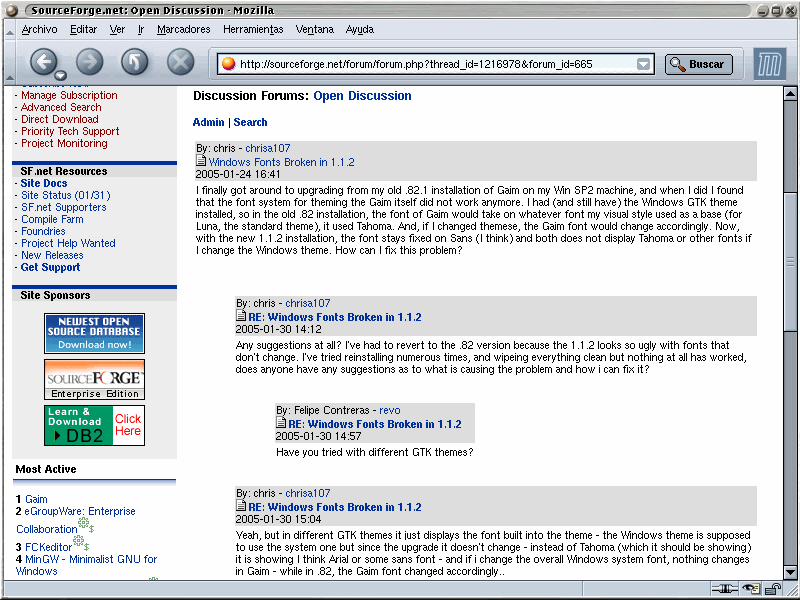
\includegraphics[bb=0 0 800 600, width=12cm, keepaspectratio]{img/foro1}
%    \caption{Página con enlaces a hilos}
%    \label{figura:foro_hilos}
% \end{figure}

%{\footnotesize
%\begin{verbatim}
%    From gaurav at gold-solutions.co.uk  Fri Jan 14 14:51:11 2005
%    From: gaurav at gold-solutions.co.uk (gaurav_gold)
%    Date: Fri Jan 14 19:25:51 2005
%    Subject: [Mailman-Users] mailman issues
%    Message-ID: <003c01c4fa40$1d99b4c0$94592252@gaurav7klgnyif>

%    Dear Sir/Madam,
%    How can people reply to the mailing list?  How do i turn off
%    this feature? How can i also enable a feature where if someone
%    replies the newsletter the email gets deleted?
%    Thanks

%    From msapiro at value.net  Fri Jan 14 19:48:51 2005
%    From: msapiro at value.net (Mark Sapiro)
%%    Date: Fri Jan 14 19:49:04 2005
 %   Subject: [Mailman-Users] mailman issues
%    In-Reply-To: <003c01c4fa40$1d99b4c0$94592252@gaurav7klgnyif>
%    Message-ID: <PC173020050114104851057801b04d55@msapiro>

%%    gaurav_gold wrote:
%    >How can people reply to the mailing list?  How do i turn off
%    this feature? How can i also enable a feature where if someone
%    replies the newsletter the email gets deleted?

%    See the FAQ
%    >Mailman FAQ: http://www.python.org/cgi-bin/faqw-mm.py
%    article 3.11
%\end{verbatim}
%}

\section{Main Objectives and Requirements}
\label{sec:objectives}

The main objective of this project is to develop a simplified \textit{reimplementation} of the Kibana web application, but at the same time, a full application with a lot of available features. All this from scratch and with our own code.

We want to build a full dashboard that allows us to manage visualizations, which data:
\begin{itemize}
    \item Will be retrieved from a \textit{no-SQL} database.
    \item Could be of any type.
    \item Will be managed in an \textit{introspective} way. Hence, we will find out the data structure that is stored in a specific moment on the database.
\end{itemize}
Given all this initial requirements, let's see in detail the project features to develop:
\begin{itemize}
    \item Building groups of data.
    \item Building summary metrics for selected visualizations.
    \item Visualizing the same data on different ways with several types of visualizations.
    \item Building visualizations for any type of data stored on the database.
    \item Allowing the user to have persistent data and save the visualizations.
    \item Allowing the user to edit or modify those visualizations, once have been created.
    \item Combining all in a customized dashboard with the same features, so we have to be able to create, save, modify and delete dashboards.
\end{itemize}
All this features has to be managed in an, easy to use, simple and intuitive user interface.

This application is required to be an \textit{SPA} or \textit{Single Page Application}, without having to install additional software on the the web browser but the web browser's standard features. Hence, we are looking for an \textit{HTML5} application that uses, as far as possible, already implemented modules in order to develop all this requirements on a "End of Degree Project" context, so we have to reuse as much components as we can.

On the other hand, we are going to work with modern frameworks such as Angular, and given the new and modern work environment that is HTML5, we are going to use recent  development methodologies and packaging technologies for applications development such as \textit{Webpack}.


%En esta sección se debería introducir la esctura de la memoria. Así:

%\begin{itemize}
%  \item En el primer capítulo se hace una intro al proyecto.

%  \item En el capítulo~\ref{chap:objetivos} (ojo, otra referencia automática) se muestran los objetivos del proyecto.

%  \item A continuación se presenta el estado del arte.

%  \item \ldots
%\end{itemize}

\section{Software Availability}
\label{sec:software-availability}
This project will be developed as an open source application and a public repository\footnote{\url{https://github.com/islimane/Angular-ElasticSearch-Dashboard_Interface}} will be created on the web-based Git repository hosting service \textit{Github}, under open source software license, so all the development history will be available. Anyone can download and install this application. In addition, we are going to build a web site\footnote{\url{https://islimane.github.io/Angular-ElasticSearch-Dashboard_Interface}} where it will be explained all our project features and where we'll apprise this application development. On the other hand, we have created and uploaded a video\footnote{\url{https://www.youtube.com/watch?v=-mal9yPCHU8&feature=youtu.be}} on \textit{youtube} showing the main features of this project.



%%%%%%%%%%%%%%%%%%%%%%%%%%%%%%%%%%%%%%%%%%%%%%%%%%%%%%%%%%%%%%%%%%%%%%%%%%%%%%%%
%%%%%%%%%%%%%%%%%%%%%%%%%%%%%%%%%%%%%%%%%%%%%%%%%%%%%%%%%%%%%%%%%%%%%%%%%%%%%%%%
% OBJETIVOS %
%%%%%%%%%%%%%%%%%%%%%%%%%%%%%%%%%%%%%%%%%%%%%%%%%%%%%%%%%%%%%%%%%%%%%%%%%%%%%%%%

\cleardoublepage % empezamos en página impar
\chapter{State of Art} % título del capítulo (se muestra)
\label{chap:state-of-art} % identificador del capítulo (no se muestra, es para poder referenciarlo)

\section{ElasticSearch} % título de sección (se muestra)
\label{sec:elasticsearch} % identificador de sección (no se muestra, es para poder referenciarla)

\textit{\textbf{Elasticsearch}} is a \textit{no-SQL} database that allows to store a big amount of data. Elasticsearch is design to be distributed, with multiple nodes working in parallel, and is design to be \textit{scalable}. The communication with this database is made by its \textit{API Rest} that works fully over \textit{HTTP}, using \textit{JSON} as document exchange format. Both the queries and the retrieved data from the Elasticsearch database is in JSON format.

\subsection{History}
\label{subsec:elasticsearch-history}
\textit{Compass} was the predecessor to Elasticsearch and it was created by \textbf{Shay Banon} in 2004. Through the implementation of the third version of Compass, came the necessity of a \textit{"scalable search solution"}. This necessity would have meant a lot of work rewriting big pieces of code, so Shay decided to build \textit{"a solution built from the ground up to be distributed"} and used a common interface, \textit{JSON} over \textit{HTTP}, available for other programming languages, and not only \textit{Java}.

The first verision of Elasticsearch was released on February 2010.

\subsection{Basic Concepts}
\label{subsec:elasticsearch-basic-concepts}

All the following concepts definitions are extracted from the Elasticsearch documentation web page\footnote{\url{https://www.elastic.co/guide/en/elasticsearch/reference/current/_basic_concepts.html}}.

\begin{itemize}
    \item \textbf{Near Realtime (NRT)}:
        Elasticsearch is a near real time search platform.
        The practical meaning of this is that there is a little latency (about one second) from the moment you store a new document, to the moment it becomes available for searching.
    \item \textbf{Index}:
        An \textbf{index} is a set of documents that share some type of characteristics. For example, you can have an index for a shop product, another index for employee data and another for bill data. An index is identified by its name (in lowercase), and this name is used for several operations as: searching, deleting, updating, etc.
    \item \textbf{Shards \& Replicas}:
        The index data can reach a large size exceeding the available physical memory.
        But this problem can be fixed by defining multiple \textbf{shards}. Each shard is a portion of data from the index data. The number of shards is defined when the index is created.

        But there is still another potential problem. It always exists the possibility to have a failure on the network system and to loose a shard/node, so it is advisable to have \textbf{replicas} of our data. A replica is a copy of the index shards.
    \item \textbf{Type}:
        We can see a \textbf{type} like an object class, with fields of different data-types.

        In Elasticsearch a type is defined by its \textit{name} and its \textit{mappings}. The \textit{mappings} are a schema of the type, where it's defined the properties that our type has, and the data-type of each property, such as \textit{integer, string, etc.}.
    \item \textbf{Document}:
        As we said about \textit{types} being like classes, we could see a \textbf{document} like a record from a single class.
        Using the same example we used for \textit{indexes}, you can have a document for a single product, another document for a single employee and yet another for a single bill.
    \item \textbf{Node}:
        We can see a \textbf{node} like a single server, as a single unit that along with other nodes, make up a cluster. This node take part on cluster's indexing and searching tasks.
    \item \textbf{Cluster}:
        As we said in the previous definition, a \textbf{cluster} is made up with multiple nodes(servers). The cluster stores all the data and allows to search and index all this data across all nodes.
        A cluster is a collection of one or more nodes (servers) that together holds your entire data and provides federated indexing and search capabilities through all nodes.
\end{itemize}


\section{Kibana}
\label{sec:kibana}

\textbf{Kibana} is an \textit{Elasticsearch} open-source plug-in. It mainly works with Elasticsearch indexed data in order to represent it into different types of visualizations such as bar charts, scatter plot charts, pie charts, ...

Kibana, as an exploration tool, can be used to log and time series analytics, application monitoring, and operational intelligence use cases.

We can find another similar applications such as \textit{Grafna}\footnote{\url{https://grafana.com/}}, \textit{incubator-superset}\footnote{\url{https://github.com/apache/incubator-superset}} and \textit{Tableau}\footnote{\url{https://www.tableau.com/}}.

\subsection{Main Features}
\label{sec:kibana-functoinalities}

In the Figure~\ref{fig:kibana-nav-bar}, we can see the Kibana's \textit{nav-bar}. Now we are going to speak about a couple of features.
\begin{figure}
  \centering
  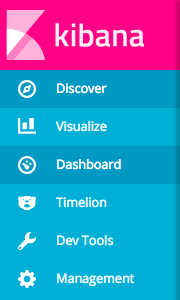
\includegraphics[height=6cm, keepaspectratio]{img/kibana-nav-bar}
  \caption{Kibana's nav-bar.}
  \label{fig:kibana-nav-bar}
\end{figure}

\begin{itemize}
    \item \textbf{Visualize}:

        \textit{Visualize} allows you to represent data with a specific type of chart. The represented data will be chosen from the available index on Elasticsearch. In addition to the Elasticsearch index, we have to choose which type of \textit{aggregations} are we going to use in order to extract our data. We can see an example on Figure~\ref{fig:kibana-visualization-example}.
        \begin{figure}
          \centering
          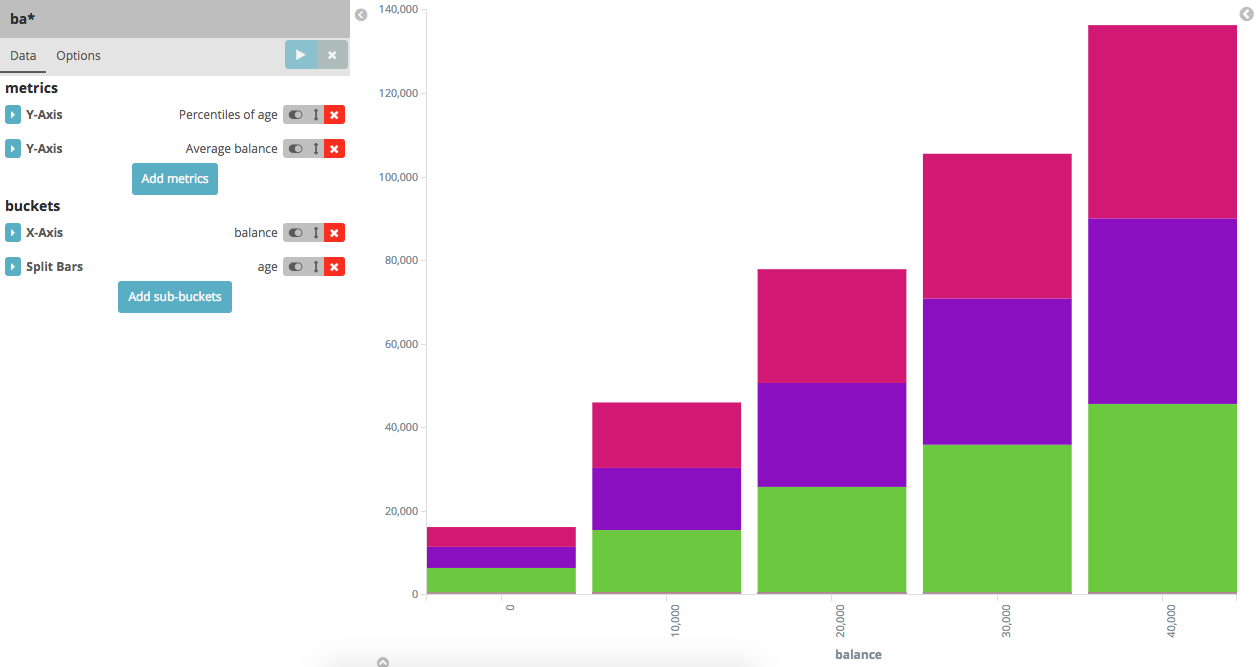
\includegraphics[width=15cm, keepaspectratio]{img/kibana-visualization-example}
          \caption{Visualization example.}
          \label{fig:kibana-visualization-example}
        \end{figure}
    \item \textbf{Dashboard}:

        The Kibana's dashboard functionality allows us to display a collection of saved visualizations and organize them by dragging and dropping. We can see an example on Figure~\ref{fig:kibana-dashboard-example}.
        \begin{figure}
          \centering
          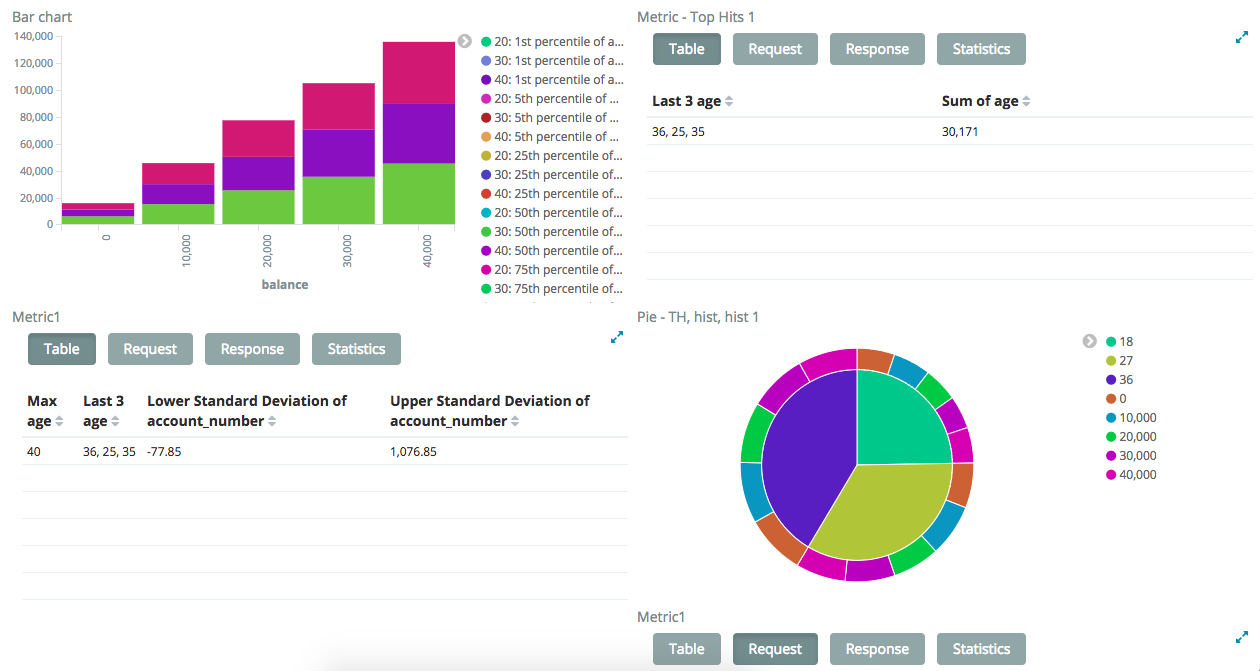
\includegraphics[width=15cm, keepaspectratio]{img/kibana-dashboard-example}
          \caption{Dashboard example.}
          \label{fig:kibana-dashboard-example}
        \end{figure}
\end{itemize}


\section{GitHub}
\label{sec:github}

"\textbf{GitHub} is a \textit{Web-based} \textbf{Git version control repository hosting service}". Github is used mainly for programming code. In addition to Git functionalities as \textit{deistributed version control} and \textit{source code management}, Github provides more features such as collaboration features for \textit{bug tracking} and for other porposes, task management, and \textit{wikis} for documentation porposes.

For the current project, a repository was created on \textit{Github} with the name of '\textit{Angular-ElasticSearch-Dashboard\_Interface}'\footnote{\url{https://github.com/islimane/Angular-ElasticSearch-Dashboard\_Interface}}.


\section{Webpack}
\label{sec:webpack}

"\textbf{Webpack} is an \textit{open-source JavaScript} module bundler". The main reason for using Webpack is to have a modular structure on your web application project. This allows you to have a cleaner code and make it more reusable and scalable.

Webpack resolves the problem of how to distribute applications and how to manage different versions while developing or distributing the application. Webpack is related with the process that gets our application \textit{minified} and with the compiling process of some programming languages into \textit{javascript} such as \textit{Typescript}. Webpack can be used from the command line and has a lot of available options to configure it through its configuration file named \textit{webpack.config.js}, also it works very well with other application environment tools such as \textit{NPM}. Webpack is a recent technology but is very demanded by web developers.

\section{Angular}
\label{sec:angular}

\textbf{Angular} is an open source \textit{web application platform} based on \textit{Typescript} and developed by Google and by a community of individuals and corporations.
Angular is commonly referred to as Angular 2.0 or later versions.

\subsection{Versions}
\label{sec:angular-versions}
Before Angular was created, there was a previous version called \textit{AngularJS} or Angular1.X. Angular was created as a complete rewrite of AngularJS.

\begin{itemize}
    \item 2.0.0:

        This was the first version of Angular. Its announcing was made at the \textit{ng-Europe} conference on September 2014. This version was build up from the ground and these were the main characteristics:
        \begin{itemize}
            \item Introduced the components hierarchy.
            \item Modules for core functionality, improving the speed of the Angular core.
            \item Possibility of using \textit{TypeScript} language. The use of this language is recommended by the Angular team.
            \item Improved \textit{dependency} injection.
            \item Dynamic loading.
            \item Reactive programming support using RxJS.
        \end{itemize}
        And much more features. The final version was released on September 14, 2016.
    \item 4.0.0:

        This version was called \textit{Angular 4} and was announced on 13 December 2016. Angular 3 was skipped due to some features already present on version 3.0.0 and to avoid confusion. This version introduced:
        \begin{itemize}
            \item \textit{Http} client.
            \item A new \textit{Rout Live Cycle}.
            \item Conditionally disable animations.
        \end{itemize}
    \item 5.0.0:

        This version was released on November 2017 and the main introduced features were:
        \begin{itemize}
            \item Support for progressive Web apps.
            \item A build optimizer and improvements related to \textit{Material Design}.
        \end{itemize}
\end{itemize}

\begin{figure}
  \centering
  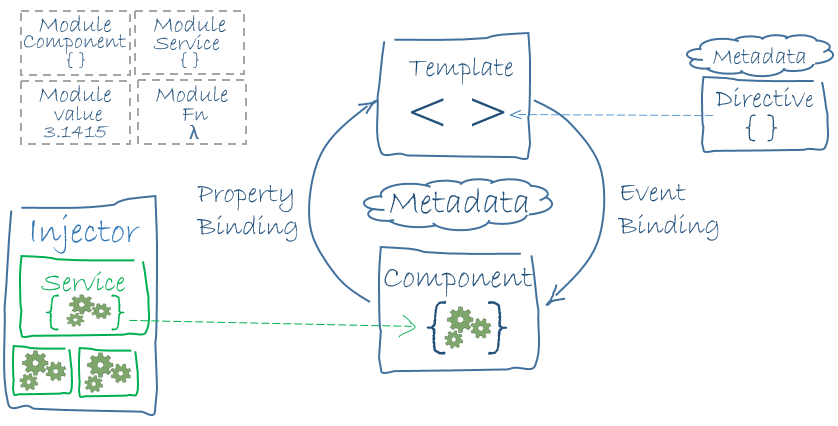
\includegraphics[width=13cm, keepaspectratio]{img/angular-architecture}
  \caption{Architecture of an Angular application}
  \label{fig:angular-architecture}
\end{figure}


\section{TypeScript}
\label{sec:typeScript}

"\textbf{TypeScript} is a free and open-source programming language developed and maintained by Microsoft. It is a strict syntactical \textit{superset} of \textit{JavaScript}, and adds optional static typing to the language".

\subsection{History}
\label{sec:typescript-history}

Before it was made public, \textit{TypeScript} gone through a two years of development process until it reached the 0.8 version. Then, was released on October 2012. Initially it had a lack of \textit{IDE} support, until 2013 when some IDE's began to have support for this language, such as \textit{Eclipse} with a dedicated pug-in, and some text editors such as \textit{Sublime}, \textit{Atom}, etc.

The reason TypeScript was created came from the necessity of a front-end programming language that fulfill the task of the development of complex and large-scale front-end applications, since JavaScript has shortcomings on that sense.

TypeScript is based on the \textit{EMACScript} approach, the reason why is because it is a standard and because it has support for \textit{class-based programming}.

\subsection{Language Features}
\label{sec:typescript-features}

\begin{itemize}
    \item Type annotations and compile-time type checking:

        TypeScript provides an optional static typing, with annotations, that is checked at compile time. If this typing it is not used, then the Javascript's dynamic typing is used. Here is an example:

        \begin{lstlisting}[language=javascript]
function planetMoons(planetName: string, moonsNum: number, spanish: boolean): any {
	if(spanish){
	    console.log('El planeta ' + planetName + ' tiene ' + moonsNum + ' lunas');
	}else{
	    console.log(planetName + '  planet has ' + moonsNum + ' moons');
	}

	return null;
}
        \end{lstlisting}
        \textit{string}, \textit{boolean} and \textit{number} are primitive types. For dynamic types it's used \textit{any}.

    \item Type inference.
    \item Type erasure.
    \item Interfaces.
    \item Enumerated type.
    \item Mixin.
    \item Generic.
    \item Namespaces.
    \item Tuple.
    \item Await.
    \item Classes (backported from EMACScript 2015).
    \item Modules (backported from EMACScript 2015).

\end{itemize}


\section{JavaScript}
\label{sec:typeScript}

"\textbf{JavaScript}, often abbreviated as JS, is a high-level, dynamic, weakly typed, prototype-based, multi-paradigm, and interpreted programming language. Alongside HTML and CSS, JavaScript is one of the three core technologies of World Wide Web content production". Generally, the main purpose of Javascript is to make pages interactive and develop online programs such as online games. Javascript is supported by most of the web browsers, for that reason, the majority of the websites employ it. There are multiple engines for Javascript, but all are standardized with the \textit{EMACScript} specification.

\subsection{History}
\label{sec:javascript-history}

Javascript came with the necessity of dynamism on web browsers. The founder of Netscape Communications, Marc Andreessen, thought that HTML needed a "glue language" to assemble component like images or plug-ins into the web markup. In 1995, Netscape Communications began to use \textit{Java} as a static programming language for Netscape Navigator, so the scripting language they had being searching for, had to be similar to Java and would complement it. Then, on May 1995, Brendan Eich wrote in 10 days this scripting language in order to compete against competing proposals. The first time this scripting language was called JavaScript was on December 1995, when the Netscape Navigator 2.0 beta 3 was released.

\subsection{Syntax}
\label{sec:javascript-syntax}

These are a few examples to illustrate the JavaScript syntax:

\begin{itemize}
    \item Variables:
        \begin{lstlisting}[language=javascript]
var x; // defines the variable x and assigns to it the special value "undefined" (not to be confused with an undefined value)
var y = 2; // defines the variable y and assigns to it the value 2
var z = "Hello, World!"; // defines the variable z and assigns to it a string entitled "Hello, World!"
        \end{lstlisting}
    \item Printing:
        \begin{lstlisting}[language=javascript]
console.log("Hello World!");
        \end{lstlisting}
    \item Functions:
        \begin{lstlisting}[language=javascript]
function add(a, b){
    return a + b;
}
add(1, 2); // returns 3
        \end{lstlisting}
\end{itemize}


\section{Lodash}
\label{sec:flexbox}

Lodash is a \textit{JavaScript} library that provides extra functions for tasks that are often required on data structure managing, a lot of them, not implemented on the main JavaScript functionality.

For example:
\begin{itemize}
    \item \textbf{\_.difference(array, [values])}: Creates an array of unique array values not included in the other provided arrays using SameValueZero for equality comparisons.
        \begin{lstlisting}[language=javascript]
_.difference([1, 2, 3], [4, 2]);
// returns [1, 3]
        \end{lstlisting}
    \item \textbf{\_.pluck(collection, path)}: Gets the property value of path from all elements in \textit{collection}.
        \begin{lstlisting}[language=javascript]
var users = [
  { 'user': 'barney', 'age': 36 },
  { 'user': 'fred',   'age': 40 }
];

_.pluck(users, 'user');
// returns ['barney', 'fred']
        \end{lstlisting}
\end{itemize}

As we can see, Lodash functions are called through the global variable "\_". All this functions can be found on the Lodash documentation\footnote{\url{https://lodash.com/docs/3.10.1}} page. This JavaScript library saves a lot of time when managing data structures.

There are other similar libraries such as \textit{UnderscoreJS}\footnote{\url{http://underscorejs.org/}}.


\section{jQuery}
\label{sec:jquery}

"\textit{jQuery} is a cross-platform JavaScript library designed to simplify the client-side scripting of HTML". jQuery it's the most used JavaScript library. jQuery's syntax is designed to make it easier to navigate a document, select DOM elements, create animations, handle events, and develop Ajax applications.

\subsection{History}
\label{sec:jquery-history}

    jQuery was originally released in January 2006 at BarCamp NYC by John Resig and was influenced by Dean Edwards' earlier cssQuery library. It is currently maintained by a team of developers led by Timmy Willison.

\subsection{Usage Examples}
\label{sec:jquery-examples}
\begin{itemize}
    \item HTML:
        \begin{lstlisting}[language=javascript]
<p>Hello</p>
        \end{lstlisting}
    \item JavaScript:
        \begin{lstlisting}[language=javascript]
$("p").clone().add( "<span>Again</span>" ).appendTo(document.body);
        \end{lstlisting}
    \item Result:

    See the result on Figure~\ref{fig:jquery-result-example}
        \begin{figure}
          \centering
          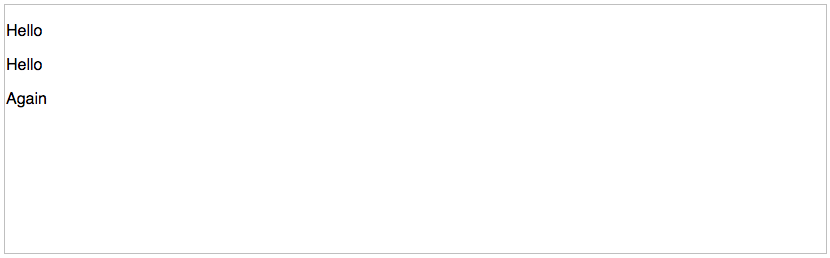
\includegraphics[width=13cm, keepaspectratio]{img/jquery-result-example}
          \caption{View result.}
          \label{fig:jquery-result-example}
        \end{figure}
\end{itemize}


\section{HTML5}
\label{sec:html5}

"\textbf{HTML5} is a markup language used for structuring and presenting content on the World Wide Web. It is the fifth and current major version of the HTML standard".

The \textit{World Wide Web Consortium} released HTML5 on October 2014, their goal was "to improve the language with support for the latest multimedia".

\subsection{Features}
\label{sec:html5-features}
These are some of the feature introduced in HTML5:
\begin{itemize}
    \item \textbf{Markup}:

        HTML5 introduces some elements that are commonly used on modern websites, they usually are replacements of old HTML elements, between these new elements we can find: \textit{<nav>}, \textit{<footer>}, \textit{<audio>}, \textit{<video>}, ...
    \item \textbf{New APIs}:

        HTML5 introduces \textit{application programming interfaces} or \textit{APIs} in addition to the markup elements that we have seen, such as \textit{Canvas}, \textit{Timed Media Playback}, \textit{Drag and Drop}, \textit{MIME type}, \textit{Web Messaging}, \textit{Web storage}, ... In this project we have mainly used \textit{Canvas} through the \textit{ChartJS} library.
\end{itemize}


\section{ChartJS}
\label{sec:chartjs}

\textbf{ChartJS} is a JavaScript library for producing dynamic, interactive data visualizations in web browsers, this is achieved by using the \textit{HTML5} \textit{canvas} element. With ChartJS you create different charts such as pie charts, bar charts, line charts, etc. You can find visual examples of each type on the ChartJS samples page\footnote{\url{http://www.chartjs.org/samples/latest/}}.

\subsection{Usage Examples}
\label{sec:chatjs-examples}

We have to instantiate the \textit{Chart} class in order to create a chart, an then assign it to a \textit{canvas} element on the DOM. The field \textit{type} indicates which chart are we going to use, and the field \textit{data} stores our chart info. Here is an example:

\begin{itemize}
    \item HTML:
        \begin{lstlisting}[language=javascript]
<canvas height='50' id='myChart' width='200'></canvas>
        \end{lstlisting}
    \item JavaScript:
        \begin{lstlisting}[language=javascript]
var ctx = document.getElementById("#myChart");
var myChart = new Chart(ctx, {
  type: 'bar',
  data: {
    labels: ["Red", "Blue", "Yellow"],
    datasets: [{
      label: '# of Votes',
      data: [12, 19, 3, 5, 2, 3],
      backgroundColor: [
        'rgba(255, 99, 132, 0.2)',
        'rgba(54, 162, 235, 0.2)',
        'rgba(255, 206, 86, 0.2)'
      ],
      borderColor: [
        'rgba(255,99,132,1)',
        'rgba(54, 162, 235, 1)',
        'rgba(255, 206, 86, 1)'
      ],
      borderWidth: 1
    }]
  }
});
        \end{lstlisting}
    \item Result:

    See the result on Figure~\ref{fig:chartjs-result-example}
    \begin{figure}
      \centering
      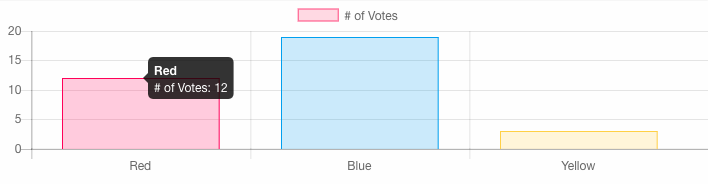
\includegraphics[width=13cm, keepaspectratio]{img/chartjs-result-example}
      \caption{View result.}
      \label{fig:chartjs-result-example}
    \end{figure}
\end{itemize}

There are a lot of libraries that allows you to render charts or graphs on a web page\footnote{\url{https://blog.sicara.com/compare-best-javascript-chart-libraries-2017-89fbe8cb112d}} such as \textit{C3.js}, \textit{Plotly.js}, etc. In this project we used ChartJS because it adapted well to the project requirements.


\section{SASS}
\label{sec:sass}

"\textbf{Sass} is a scripting language that is interpreted or compiled into \textit{Cascading Style Sheets} (CSS)". Sass uses two types of syntax. The first is original syntax, similar to \textit{Haml}\footnote{\url{https://en.wikipedia.org/wiki/Haml}}. The second is \textit{SCSS}, a syntaxt that uses blocks formatting like \textit{CSS}

\subsection{Features}
\label{sec:sass-features}
\begin{itemize}
    \item \textbf{Variables}:

        Sass allows defining variables using a dollar sign (\$).
        \begin{lstlisting}[language=javascript]
$primary-color: #3bbfce;

.content-navigation {
  border-color: $primary-color;
  color: darken($primary-color, 10%);
}
        \end{lstlisting}

    \item \textbf{Block Nesting}:

        Sass allows nesting different style blocks, this a improves the code structure, makes it more readable and saves lines of code.
        \begin{lstlisting}[language=javascript]
table.hl {
  margin: 2em 0;
  td.ln {
    text-align: right;
  }
}
        \end{lstlisting}

    \item \textbf{Loops}:

        With Sass you can create loops of style blocks, this feature helps to save code when you have similar \textit{id's} or \textit{classes}. Her is an example:
        \begin{lstlisting}[language=javascript]
$squareCount: 3
@for $i from 1 through $squareCount
  #square-#{$i}
   background-color: red
   width: 50px * $i
   height: 120px / $i
        \end{lstlisting}

    \item There are more Sass features such as \textit{arguments}, \textit{selector inheritance}, ... All of these features can be found on the Sass documentation web page\footnote{\url{http://sass-lang.com/documentation/file.SASS_REFERENCE.html}}.
\end{itemize}


\section{Flexbox}
\label{sec:flexbox}

"The \textit{CSS3 Flexible} Box, or \textbf{Flexbox}, is a layout mode intended to accommodate different screen sizes and different display devices". Flexbox is very useful when you have to organize your application view, so for example, sticking a \textit{footer} to the bottom of a page, designing a \textit{navigation bar}, creating a custom grid, ... is much easier using Flexbox.

Related to the Flexbox concept, it allows to manage an element width and the height to improve its fitting in the available space on the display regardless of the device that is being used. This elements are shrunken to prevent overflow or expanded to fill remaining space.

\subsection{Usage Examples}
\label{sec:chatjs-examples}

In order to use Flexbox styles, we have to apply the style "\textit{display: flex}" in our container element. Let's see a few Flexbox usage examples.

\begin{itemize}
    \item \textbf{flex-wrap}:

        Defines if flexbox items appear on a single line or on multiple lines within a flexbox container.
        \begin{lstlisting}[language=javascript]
flex-wrap: nowrap;
flex-wrap: wrap;
        \end{lstlisting}
        \begin{figure}
          \centering
          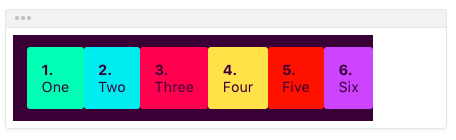
\includegraphics[width=11cm, keepaspectratio]{img/no-wrap-example}
          \caption{no-wrap example.}
          \label{fig:no-wrap-example}
        \end{figure}
        \begin{figure}
          \centering
          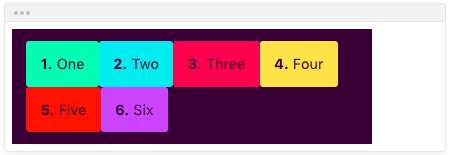
\includegraphics[width=11cm, keepaspectratio]{img/wrap-example}
          \caption{wrap example.}
          \label{fig:wrap-example}
        \end{figure}

    \item \textbf{justify-content}:

        Defines how flexbox items are aligned according to the main axis, within a flexbox container.
        \begin{lstlisting}[language=javascript]
justify-content: flex-end;
justify-content: center;
        \end{lstlisting}
        \begin{figure}
          \centering
          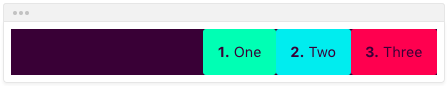
\includegraphics[width=11cm, keepaspectratio]{img/flex-end-example}
          \caption{flex-end example.}
          \label{fig:flex-end-example}
        \end{figure}
        \begin{figure}
          \centering
          
\includegraphics[width=11cm, keepaspectratio]{img/center-example}
          \caption{center example.}
          \label{fig:center-example}
        \end{figure}
\end{itemize}


%%%%%%%%%%%%%%%%%%%%%%%%%%%%%%%%%%%%%%%%%%%%%%%%%%%%%%%%%%%%%%%%%%%%%%%%%%%%%%%%
%%%%%%%%%%%%%%%%%%%%%%%%%%%%%%%%%%%%%%%%%%%%%%%%%%%%%%%%%%%%%%%%%%%%%%%%%%%%%%%%
% ESTADO DEL ARTE %
%%%%%%%%%%%%%%%%%%%%%%%%%%%%%%%%%%%%%%%%%%%%%%%%%%%%%%%%%%%%%%%%%%%%%%%%%%%%%%%%

%\cleardoublepage
%\chapter{Estado del arte}

%Descripción de las tecnologías que utilizas en tu trabajo.
%Con dos o tres párrafos por cada tecnología, vale.
%Se supone que aquí viene todo lo que no has hecho tú.

%Puedes citar libros, como el de Bonabeau et al. sobre procesos estigmérgicos~\cite{bonabeau:_swarm}. % Nota que el ~ añade un espacio en blanco, pero no deja que exista un salto de línea. Imprescindible ponerlo para las citas.

%También existe la posibilidad de poner notas al pie de página, por ejemplo, una para indicarte que visite la página de LibreSoft\footnote{\url{http://www.libresoft.es}}.

%\section{Sección 1}
%\label{sec:seccion1}

%Hemos hablado de cómo incluir figuras.
%Pero no hemos dicho nada de tablas.
%A mí me gustan las tablas.
%Mucho.
%Aquí un ejemplo de tabla, la Tabla~\ref{tabla:ejemplo}.

%\begin{table}
 %\begin{center}
%  \begin{tabular}{ | l | c | r |} % tenemos tres colummnas, la primera alineada a la izquierda (l), la segunda al centro (c) y la tercera a la derecha (r). El | indica que entre las columnas habrá una línea separadora.
%    \hline
%    1 & 2 & 3 \\ \hline % el hline nos da una línea vertical
%    4 & 5 & 6 \\ \hline
%    7 & 8 & 9 \\
%    \hline
%  \end{tabular}
%  \label{tabla:ejemplo}
%  \caption{Ejemplo de tabla}
% \end{center}
%\end{table}



%%%%%%%%%%%%%%%%%%%%%%%%%%%%%%%%%%%%%%%%%%%%%%%%%%%%%%%%%%%%%%%%%%%%%%%%%%%%%%%%
%%%%%%%%%%%%%%%%%%%%%%%%%%%%%%%%%%%%%%%%%%%%%%%%%%%%%%%%%%%%%%%%%%%%%%%%%%%%%%%%
% DISEÑO E IMPLEMENTACIÓN %
%%%%%%%%%%%%%%%%%%%%%%%%%%%%%%%%%%%%%%%%%%%%%%%%%%%%%%%%%%%%%%%%%%%%%%%%%%%%%%%%

\cleardoublepage
\chapter{Development}

\section{SCRUM Methodology}
\label{sec:scrum}

\textbf{SCRUM} is a work methodology designed mainly for \textit{software development}. The main philosophy of this methodology consists in subdividing the work into groups of smaller tasks, each group is called "\textit{Sprint}".

"Scrum is an iterative and incremental agile software development framework for managing product development".

A key principle of Scrum is the dual recognition:
\begin{itemize}
    \item Customers decision may change during the sprint development process (requirements volatility).
    \item There will be unpredictable challenges—for which a predictive or planned approach is not suited.
\end{itemize}

In the \textit{SCRUM} framework we can find three main roles:
\begin{itemize}
    \item \textbf{Product owner}: Ensures that the team delivers value to the business and represents both the product's stakeholders and the voice of the customer. The product owner manage the work process defining the product, adding stories to the backlog and prioritizing work.
    \item \textbf{Development team}: The team is the one that completes the tasks of a Sprint, building the product increments.
    \item \textbf{SCRUM master}: Removes the impediments, allowing the team to deliver product goals. The SCRUM master  filters all distracting influences from the development team.
\end{itemize}

On Figure~\ref{fig:scrum-framework} we can see a general SCRUM framework.
\begin{figure}
  \centering
  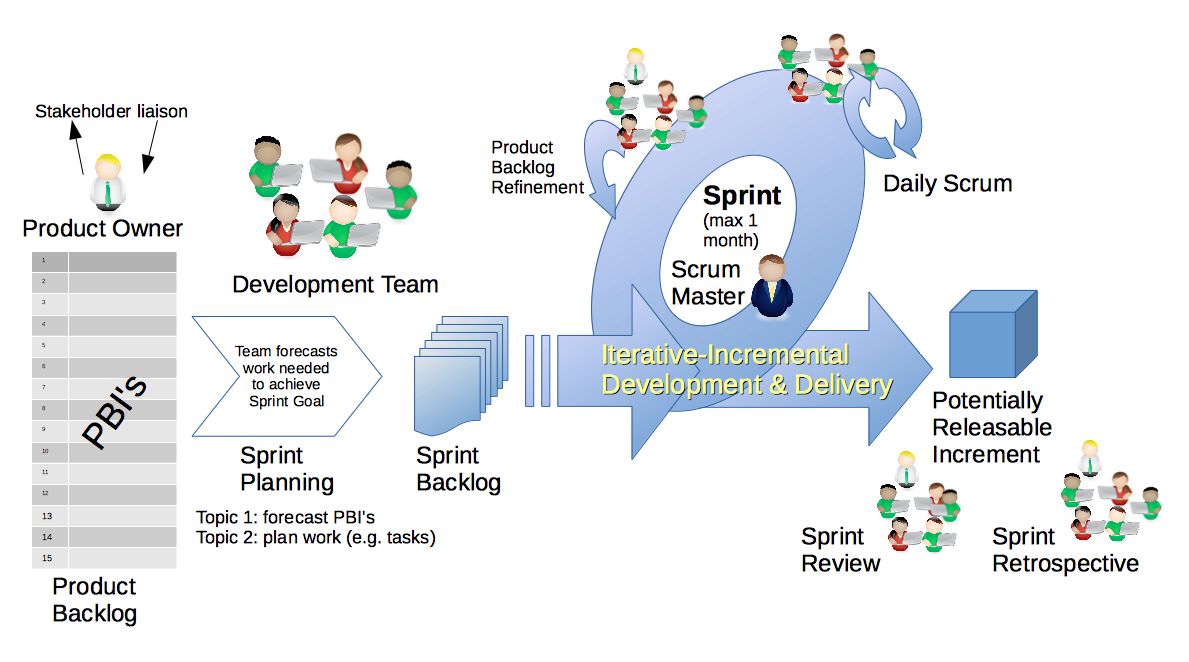
\includegraphics[width=14cm, keepaspectratio]{img/Scrum_Framework}
  \caption{SCRUM Framework}
  \label{fig:scrum-framework}
\end{figure}


\section{Sprint 1}
\label{sec:sprint-1}

\subsection{Key Objectives}
\label{sec:key-objectives}

The main goals or tasks for this sprint are:
\begin{itemize}
    \item Basic Elasticsearch interface which allows to visualize a simple metric. The data must come from Elastcsearch through an API request.
    \item Include more aggregation options and Index selecting functionality.
\end{itemize}

\subsection{Implementing a simple metric request}
\label{sec:simple-request}
We are at the beginning of this project, so the first thing we are going to do is to connect our Angular project to Elasticsearch. This can be achieved by installing the Elasticsearch library\footnote{\url{https://github.com/elastic/elasticsearch-js}} for Angular. This library will allow us to make requests to Elasticsearch through its javascript API.

We need an Elasticsearch client instance, this instance will give us the access to the Elasticsearch API. Elasticsearch, by default, it listens on the '9200' port, so we'll need to specify it too.
\begin{lstlisting}[language=javascript, caption=Client Instance, label=code:client-instance]
export class Elasticsearch {
	public clientElasticsearch: Client;
	constructor() {
		this.clientElasticsearch = new Client({
			host: 'localhost:9200',
			log: 'trace' // This is for debug purposes
		});
	}
...
}
\end{lstlisting}
This Elasticsearch class is created as an Angular \textbf{service}. In Angular, services are usually used for fetching data from the outside, this is what we are trying to achieve.

The next thing we are going to do is to request a simple "count" from Elasticsearch. In order to achieve this goal, we need to specify an Elasticsearch \textbf{index}.
\begin{lstlisting}[language=javascript]
...
public count(index): PromiseLike<number> {
	return this.clientElasticsearch.count({
			index: index
	}).then(
		response => response.count,
		this.handleError
	);
}
...
\end{lstlisting}
Now we just need to display the response.
\begin{lstlisting}[language=javascript]
// Html
<button (click)="displayData()">Display</button>
Count: <span>{{data}}</span>

// Typescript
...
data: number = 0;
...
displayData(): void {
	this.elasticsearch.count('bank')
	.then(count => this.data = count);
}
...
\end{lstlisting}


\subsection{Adding aggregations and dynamic index}
\label{sec:adding-aggregations}
First, in order to fetch the available indexes we are going to use the "cat" request, supported by the javascript API.
\begin{lstlisting}[language=javascript]
...
public getIndices(): PromiseLike<string[]>{
     return this.clientElasticsearch.cat.indices({
     	format: 'json'
     })
...
\end{lstlisting}
This method returns a JSON object, as we have specified in the "format" field. So we just need to parse this JSON response in order to build our indexes array. The next step is to retrieve all "number" fields for each index, since we are not going to implement aggregations that need another field type yet.
\begin{lstlisting}[language=javascript]
...
public getIndexNumFields(index): PromiseLike<string[]> {
 		return this.map(index).then(function(response){
...
\end{lstlisting}
The map method returns the index mappings, which we need to parse in order to build our "number fields" array.

The \textbf{PromiseLike} class is very useful because allows us to wait until the request is finished, in order to execute the appropriate callback function and manage the retrieved data asynchronously.

For now, we are going to include functionality for aggregations, which only works with fields of type "number". To achieve this we are going to use the "search" request provided by the Elasticsearch javascript API. This request returns a JSON object which we need to parse in a different way depending on the aggregation we are requesting, in order to get a displayable result.
\begin{lstlisting}[language=javascript]
...
// avg, sum, min, max, median, std_deviation, unique_count
public numFieldCalculation(index: string, aggs: any): PromiseLike<any>{
	return this.clientElasticsearch.search({
			"index": index,
			"body": {"size": 0, "aggs": aggs}
	})
...
\end{lstlisting}

The final stage view at the end of this sprint is shown on Figure~\ref{fig:sprint1-final-stage}.
\begin{figure}
  \centering
  \includegraphics[width=13cm, keepaspectratio]{img/final-stage-sprint1}
  \caption{Final stage view - Sprint 1}
  \label{fig:sprint1-final-stage}
\end{figure}

For a better understanding, a general architecture for this sprint is shown on Figure~\ref{fig:sprint1-architecture}.
\begin{figure}
  \centering
  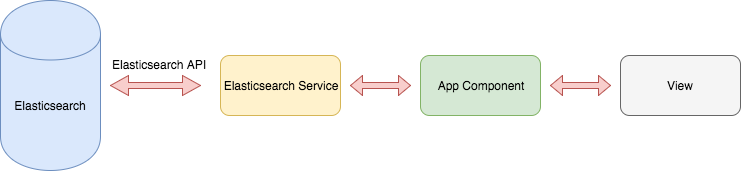
\includegraphics[width=13cm, keepaspectratio]{img/sprint1_architecture}
  \caption{Sprint 1 architecture.}
  \label{fig:sprint1-architecture}
\end{figure}


\section{Sprint 2}
\label{sec:sprint-2}
\subsection{Key Objectives}
\label{sec:key-objectives}

The main goals or tasks for this sprint are:
\begin{itemize}
    \item Finish metrics functionality implementation.
    \item Implement Data Table visualization functionality.
    \item Load multiple metrics or buckets and changing between visualizations, both dynamically.
    \item Allow to load and save visualizations.
\end{itemize}

\subsection{Finishing metrics}
\label{sec:finishing-metrics}
Following the same logic as we did with the previous aggregations, we implement 'Percentiles', 'Percentile Ranks' and 'Top Hit' aggregations. The complexity of this aggregations is a little bit higher because this aggregations need more data in order to perform the request.

For this reason, we are going to have individual components for each one of this aggregations and a general \textit{metrics component} for the other aggregations since they share the main calculation logic.

The architecture on Figure~\ref{fig:sprint2-architecture-1} shows how remains the general structure. And the final version of a metric example is shown on Figure~\ref{fig:metric-count-calcuation}.
\begin{figure}
  \centering
  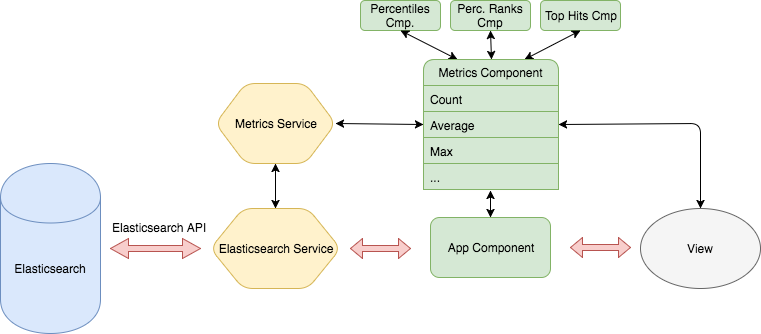
\includegraphics[width=13cm, keepaspectratio]{img/sprint2_architecture_1.png}
  \caption{Sprint 2 architecture - Step 1.}
  \label{fig:sprint2-architecture-1}
\end{figure}

\subsection{Implementing "Data Table" feature}
\label{sec:data-table-feature}
In relation with the "Data Table" visualization implementation we followed the same structure as we did with the "Metric" visualization. The main difference here is the way we structure the data in order to display it in a table.

Another important difference with the "Metric" visualization is the introduction of Elasticsearch \textbf{buckets}. Because of the way "Data Table" visualizations work, Elasticsearch returns the requested data in groups of results, depending on the "bucket aggregation" that has been selected. For this project we are going to use two different bucket aggregations between all the possible aggregations:
\begin{itemize}
    \item Histogram
    \item Range
\end{itemize}

Here the complexity of the requests grows. Because of this complexity, we are going to use a javascript library called "\textbf{bodybuilder}"\footnote{\url{https://github.com/danpaz/bodybuilder}}. As we could understand by its name, this library helps us to build the request bodies. For example if we want to make a simple count over an index, and retrieve the data as "histogram buckets" with an interval we would do the following:
\begin{lstlisting}[language=javascript]
// Builder process
bodybuilder().aggregation('histogram', null, 'bucket_1', {
  	field: 'age',
	interval: 5
}).build()

// Result
{
  "aggs": {
    "bucket_1": {
      "histogram": {
        "field": "age",
        "interval": 5
      }
    }
  }
}
\end{lstlisting}

A final version of a Data Table visualization example is shown on Figure~\ref{fig:data-table-multiaggregation-calculation}.

\subsection{Load multiple metrics or buckets and changing between visualizations, both dynamically}
\label{sec:loading-dynamically}
During the implementation of this project we found several issues using the Angular live-cycle hook in order to load, create, delete or modify components dynamically, specially when the component had a complex structure. For this reason we decided to have a dedicated component that allows us to complete all this tasks. We named this component "DynamicComponent".

This dynamic component works as a container for a single component or for multiple components.

Let's see the component's API:
\begin{lstlisting}[language=javascript]
// This method allows us to insert one or more components, it requires:
// - uniqueId: to store the component in a map for future modifications or access.
// - inputs: an object with the component parameters values.
// - events: an array with the event names we want to listen from this component.
// - componentType: the component type we want to instantiate.
addComponent(uniqueId: string, inputs: any, events: Array<string>, componentType: any): any{};

// this method is already executed on the addComponent(), but we may need it after the component initialization to modify some component parameter
setInputs(uniqueId:string, inputs: any): void{};

// This method destroys a loaded component by its unique ID
destroyCmp(uniqueId: string): void{};
\end{lstlisting}

Due to the Angular live-cycle hook behaviour we have commented before, we need a more efficient way to set specific component parameters. Usually when a parent component needs to pass parameters to a child component, we get it done by adding attributes on the child component selector, but due to the complexity of the bucket and metric components, the Angular live-cycle hook was acting erratically and breaking the parent-child parameters synchronization. We needed to communicate with grandchildren components too and this was bringing on more synchronization problems.

For this reason, we used a different technique for communicating a parent with its children or grandchildren components or even another component without direct relationship. This approach for communicating components is made via \textbf{service}, we can see a diagram on Figure~\ref{fig:parent-child-via-service}.
\begin{figure}
  \centering
  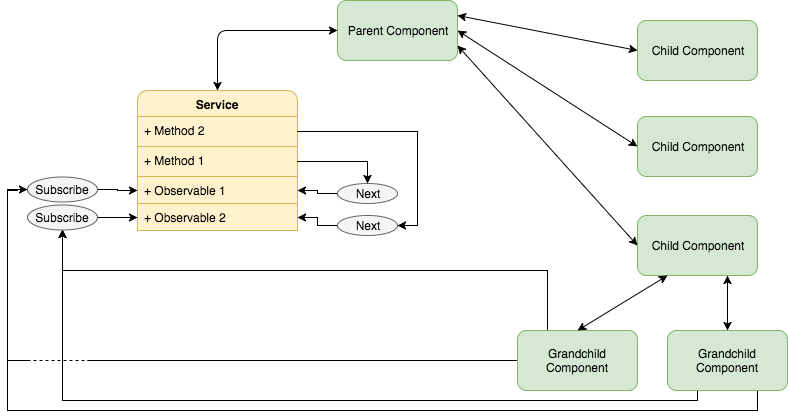
\includegraphics[width=13cm, keepaspectratio]{img/parent-child-via-service.png}
  \caption{Components communication via Service.}
  \label{fig:parent-child-via-service}
\end{figure}

As we can see on Figure~\ref{fig:parent-child-via-service}, a "Parent Component" communicates with its grandchildren employing \textbf{observable} variables declared on a \textbf{service}, each time a method executes "\textbf{next}" on a observable, a callback function is executed on each grandchild that was subscribed to this observable accessing the sent data.

To give an example, we can see this technique the following components:
\begin{itemize}
    \item \textbf{VisualizationsComponent}: acting as a "Parent Component".
    \item \textbf{VisualizationsService}: acting as the communicating service.
    \item \textbf{BucketsComponent}: acting as a "Grandchild Component".
\end{itemize}

Another advantage of this technique appears when we need a bidirectional communication between components, in this case we wouldn't need \textit{input} variables or component events.


\subsection{Loading and saving visualizations}
\label{sec:loading-and-saving}
At this point we are able to create two types of visualizations, "Metric" and "Data Table", but we are still not able to store them in Elasticsearch neither loading saved visualizations.

To achieve this goals we have to create a new Elasticsearch index which will store all visualizations data. The name of this index we'll be "sakura".

Now we need a \textit{type} which will define what data represents our visualizations.

Our index mapping looks like this:
\begin{lstlisting}[language=javascript]
visualization: {
    properties: {
        kibanaSavedObjectMeta: {
            properties: {
                searchSourceJSON: {
                    type: "text",
                    fields: {
                        keyword: {
                            type: "keyword",
                            ignore_above: 256
                        }
                    }
                }
            }
        },
        title: { type: "text" },
        visState: { type: "text" }
    }
}
\end{lstlisting}

Each field stores specific data in order to load a visualization:
\begin{itemize}
    \item \textbf{kibanaSavedObjectMeta}: data related with the visualization index.
    \item \textbf{title}: visualization's title.
    \item \textbf{visState}: data related with the aggregations.
\end{itemize}

Once we've created the visualization object, the saving process consists of 2 steps:
\begin{itemize}
    \item Checking if there is already a visualization on Elasticsearch with the same id (title).
    \item If there is already a visualization, updating it, otherwise creating a new one.
\end{itemize}

In Elasticsearch we use the "search" action in order to look for a document:
\begin{lstlisting}[language=javascript]
this.cli.search({
		"index": '.sakura',
		"type": type,
		"body": body
})
\end{lstlisting}

In this case the type is "visualization" and the body is build in the following way:
\begin{lstlisting}[language=javascript]
bodybuilder().filter('term', '_id', title).build();
// Returns:
{
  "query": {
    "bool": {
      "filter": {
        "term": { "_id": title }
      }
    }
  }
}
\end{lstlisting}

To create a document we use the "create" action:
\begin{lstlisting}[language=javascript]
this.cli.create({
	index: index,
	type: type,
	id: id,
	body: body
})
\end{lstlisting}

And we use "update" to modify an existing document:
\begin{lstlisting}[language=javascript]
this.cli.update({
	index: '.sakura',
	type: type,
	id: id,
	body: { doc: doc }
})
\end{lstlisting}

The general structure at the end of this sprint is shown on Figure~\ref{fig:sprint2-architecture-2}.
\begin{figure}
  \centering
  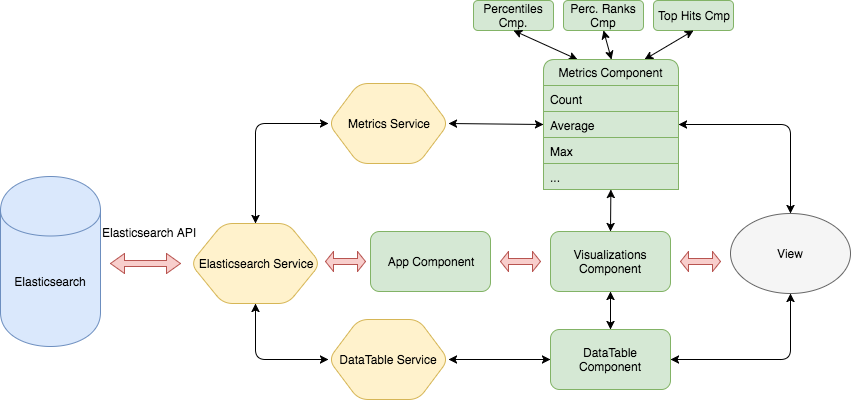
\includegraphics[width=13cm, keepaspectratio]{img/sprint2_architecture_2}
  \caption{Sprint 2 final structure.}
  \label{fig:sprint2-architecture-2}
\end{figure}


\section{Sprint 3}
\label{sec:sprint-3}

\subsection{Key Objectives}
\label{sec:key-objectives}
The main goals or tasks for this sprint are:
\begin{itemize}
    \item Implement "Pie Chart" visualization.
    \item Implement "Bar Chart" visualization.
    \item Design the application user interface.
    \item Implement deleting feature for visualizations.
\end{itemize}

\subsection{Implementing the "Pie Chart"}
\label{sec:pie-chart}
For this visualization we'll need a library that provides us chart features and allows us to display a "Pie Chart". In this case we decide to use \textit{ChartJS}.

ChartJS provides a dedicated module for Angular but it has some defects and limitations and still needs improvements, for this reason we decide to import the ChartJS library directly to the HTML and arrange each chart to the HTML through \textit{jQuery}.

For this visualizations, the process complexity of request body building, and the process complexity of response parsing are much higher compared to the visualization types already implemented.

The request body has the following format:
\begin{lstlisting}[language=javascript]
-> aggs
    ++ bucket_1
        ** aggs
            >> metric_aggregation
            >> bucket_2
                ## aggs
                    ~~ metric_aggregation
                    ~~ bucket_3
                        -- ... // keeps going on with until we reach the desired number of levels
                ## bucket_aggregation_2
        ** bucket_aggregation_1
\end{lstlisting}

As we can see, each bucket object contains the selected metric, and this metric is the same for every bucket.

The Elasticsearch response object doesn't fit at all with the way we want to display the received data, so we need to parse it into a more "friendly" object in order to make it easy creating the required data in order to render the chart with ChartJS. The parsed object will have the following format:
\begin{lstlisting}[language=javascript, caption=Custom results object, label=code:cutom-pie-chart-obj]
// This map contains the bucket(level) id as key and the array of results as value.
-> Map<String, Array<any>>
    ++ bucket_1
        ** [{result_obj_1}, {result_obj_2}, {result_obj_3}, ...]
    ++ bucket_2
        ** [{result_obj_1}, {result_obj_2}, {result_obj_3}, ...]
    ...

\end{lstlisting}

To display a "Pie Chart" we have a canvas element which we have to reference from our component.
\begin{lstlisting}[language=javascript]
<canvas baseChart id="myChart"></canvas>
\end{lstlisting}
The chart object is formed by the following fields:
\begin{itemize}
    \item \textbf{type}: In this case this is 'pie'.
    \item \textbf{data}: This will contain our \textbf{datasets} with the pie data defining each one of the different levels that forms our "Pie Chart".
    \item \textbf{options}: This defines our chart configuration an characteristics such us responsiveness, tooltip customization, etc.
\end{itemize}

Each \textbf{dataset} defines a different level on our "Pie Chart" and it's formed by the following fields:
\begin{itemize}
    \item \textbf{data}: An array of values where each value appertain to a slice of the current level. Examples of this array are shown on code snippet ~\ref{code:cutom-pie-chart-obj}.
    \item \textbf{backgroundColor}: An array of hexadecimal colors for each slice of the current level. This array is created randomly, the way we created this array is keeping and array of colors that are already displayed and calculating a given distance between hexadecimal colors in a decimal form, thus we ensure that all colors will differ one from each other.
    \item \textbf{labels}: An array of labels with value information for each slice of the current level. Here we had to use a library named "text-table". The reason we need this library is because ChartJS doesn't take \textit{HTML} code in order to display a label but it takes a simple \textit{String}, in this case we need to display a table within the label, since each row will represent an upper level, so this library parses an array of arrays and convert it into a table in a \textit{String} format with "line breaks".
\end{itemize}

A final version of a Pie Chart visualization example is shown on Figure~\ref{fig:pie-chart-calculation}.

\subsection{Implementing the "Bar Chart"}
\label{sec:pie-chart}

For this visualization we are also using ChartJS.

The request and response objects have the same complexity as the request and response objects for the "Pie Chart" visualization.

For the "Bar Chart" visualization, the request body is not as complex as the "Pie Chart" visualization request but still has some complexity. Let's see its format:
\begin{lstlisting}[language=javascript, caption=Bar Chart request body format, label=code:bar-chart-request]
-> aggs
    ++ bucket_1
        ** aggs
            ~~ metric_aggregation_1
            ~~ metric_aggregation_2
            ~~ ...
        ** bucket_aggregation_1
\end{lstlisting}

As we can see there is just a single bucket and over it we are going to calculate one or more metric aggregations.

In this case we have to parse the response object into an object with a more "friendly" data structure like we did before with the "Pie Chart" visualization response. This new object has the following format:
\begin{lstlisting}[language=javascript, caption=Custom results object, label=code:cutom-pie-chart-obj]
// This map contains the metric result label as key and the array of results as value.
-> Map<String, Array<any>>
    ++ metric_result_label_1
        ** [{result_obj_1}, {result_obj_2}, {result_obj_3}, ...]
    ++ metric_result_label_2
        ** [{result_obj_1}, {result_obj_2}, {result_obj_3}, ...]
    ...
\end{lstlisting}

Each result object for a metric aggregation appertains to a bucket value, so that if we have 5 results for the requested bucket, we'll have 5 bars containing a single result from each requested metric.

To display a "Bar Chart" we are going to use the same method as we did before with the "Pie Chart" visualization.

The \textit{Chart} object contains the same fields we mentioned earlier, but now we set the \textit{type} to 'bar'.

The \textit{dataset} object is now much simpler, now it only contains information for a single result, so this is how remains:
\begin{itemize}
    \item \textbf{data}: An array of values for each slice of the current level. Examples of this array are shown on code snippet ~\ref{code:cutom-pie-chart-obj}.
    \item \textbf{backgroundColor}: A single hexadecimal color. This will be calculated randomly using the same logic as we did with the "Pie Chart".
    \item \textbf{labels}: A single \textit{string} value which identifies the current values collection.
\end{itemize}
A final version of a Bar Chart visualization example is shown on Figure~\ref{fig:bar-chart-calculation}.

\subsection{Designing a user interface}
\label{sec:pie-chart}

We have reached a point on the development process where it would be great to have a more intuitive, colorful and dynamic user interface.

For now we only have one view,  "Visualizations", so we are going to design a user interface thinking on elements that we already have and their functionality.

On Figure~\ref{fig:user-interface-mockup} we can see the mock-up schema we want to get implemented.
\begin{figure}
  \centering
  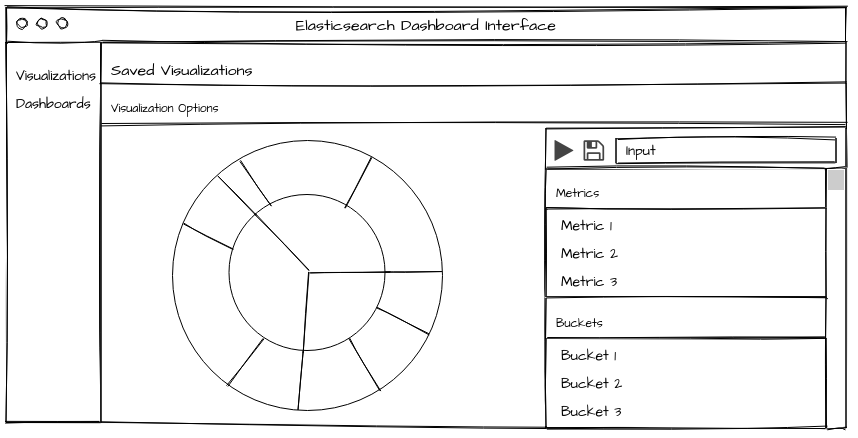
\includegraphics[width=15cm, keepaspectratio]{img/user_interface_mockup}
  \caption{Use Interface mock-up}
  \label{fig:user-interface-mockup}
\end{figure}

To get all elements in their right position, such as the nav-bar or the metrics and buckets side-bar we are going to use \textbf{Flexbox}.

The tough task comes when we have to implement the metrics and buckets window. As we can see, it has a \textit{scroll-bar} and the window is not positioned on the top of the page, it position depends always on the elements above it, and this elements can expand when we click on them, so the metrics and buckets window needs a dynamic height.

We achieve this dynamic height by employing two things: Angular dynamic attributes and \textit{jQuery}.

As we can see bellow, the attribute takes a dynamic value through the \textit{getHeight()} function, this function receives the element \textit{id} as a parameter in order to reference it later with \textit{jQuery}:
\begin{lstlisting}[language=javascript, caption=Dynamic height with Angular, label=code:angular-dynamic-heigh]
<div
    id="metricsAndBuckets"
    [style.height.px]="_getHeight('metricsAndBuckets')">
        <metrics ...></metrics>
        <buckets ...></buckets>
</div>
\end{lstlisting}

Bellow we can see how the function calculates the element's height give the current window height and the current top position of our element:
\begin{lstlisting}[language=javascript, caption=Dynamic height with Angular, label=code:cutom-pie-chart-obj]
private _getHeight(elemId: string): Number {
	let configHeight = ($(window).height() - $('#' + elemId).position().top);
	return configHeight;
}
\end{lstlisting}

Setting this height to our element and giving it a "\textit{overflow-x: scroll;}" style, we make this window "\textit{scrollable}".

To achieve the expandable panels for "Saved Visualizations" and "Visualization Options" we used a dynamic style and a \textit{click} event, this process is similar to the dynamic height process we have shown before.

All icons are extracted from the \textit{font-awesome} library. On Figure~\ref{fig:final-user-interface} we can see a final view of our user interface, with the same visualization example as in the mock-up schema.
\begin{figure}
  \centering
  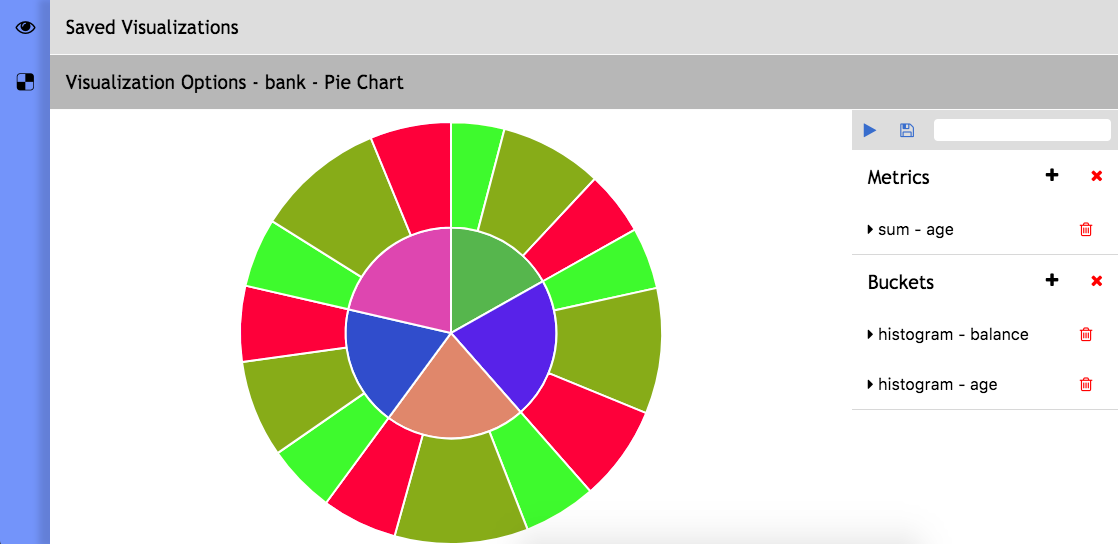
\includegraphics[width=15cm, keepaspectratio]{img/final-user-interface.png}
  \caption{Final User Interface}
  \label{fig:final-user-interface}
\end{figure}

\subsection{Deleting visualizations}
\label{sec:deleting-visualizations}
To achieve the visualization deleting process, we are going to use another Elasticsearch action named "delete".
\begin{lstlisting}[language=javascript, caption=Calling the Elasticsearch "delete" action, label=code:elasticsearch-delete]
public deleteDoc(type: string, id: string): PromiseLike<any>{
	return this.cli.delete({
		index: '.sakura',
		type: type,
		id: id,
		refresh: 'wait_for'
	})...
}
\end{lstlisting}

As we can see, we have to pass the document "type" and the document "id". The "\textit{refresh: 'wait\_for'}" option allows as to wait until the action has finish in order to refresh the saved visualizations panel and make the deleted visualization disappear.


\section{Sprint 4}
\label{sec:sprint-4}

\subsection{Key Objectives}
\label{sec:key-objectives}
\begin{itemize}
    \item Implement a dashboard user interface capable of showing multiple saved visualizations.
    \item Implement the saving, modifying and deleting features for dashboards .
\end{itemize}

\subsection{Implementing the visualizations dashboard}
\label{sec:visualizations-dashboard}
Once we've finished the "Visualizations" section, we are going to reuse our visualization components in order to make a "\textit{customizable}" dashboard interface.

First of all, we have to be able to change between the sections "Visualizations" and "Dashboards", to achieve this we are going to use the Angular \textbf{routing} feature. This feature allows us to navigate between different application content. To achieve this we have to import the following modules:
\begin{lstlisting}[language=javascript, caption=Paths definition, label=code:dashboard-object]
const routes: Routes = [
	{ path: '', redirectTo: '/visualizations', pathMatch: 'full' },
	{ path: 'visualizations',	component: VisualizationsComponent },
	{ path: 'dashboards',	component: DashboardsComponent }
];
\end{lstlisting}

Then we have to specify which path corresponds to each component, and a default component when we launch the application:
\begin{lstlisting}[language=javascript, caption=Routing modules, label=code:dashboard-object]
import { RouterModule, Routes } from '@angular/router';
\end{lstlisting}

To implement our dashboard grid where our visualizations will be shown we are using an angular module named "\textit{angular2gridster}"\footnote{\url{https://github.com/swiety85/angular2gridster}}. This module will allow us to:
\begin{itemize}
    \item Drag and drop visualizations containers.
    \item Store the position, size and another useful data for each visualization container.
\end{itemize}

On Figure~\ref{fig:dashboards-diagram} we can see how this module fits in our dashboard.
\begin{figure}
  \centering
  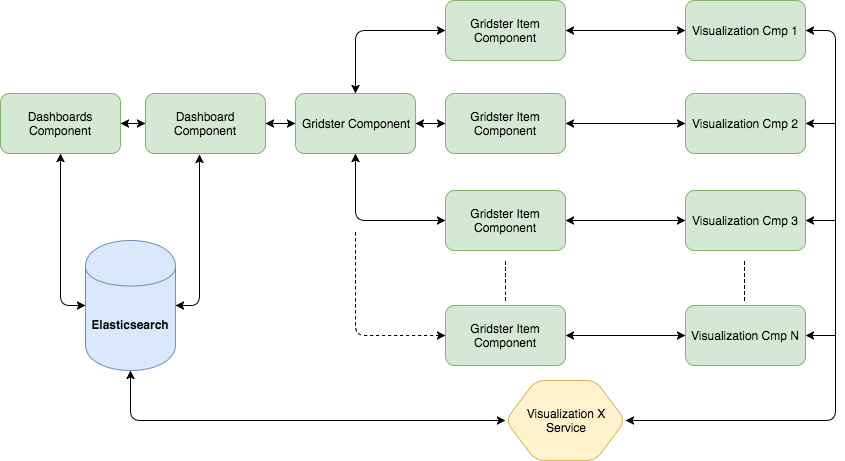
\includegraphics[width=15cm, keepaspectratio]{img/dashboards-diagram}
  \caption{Dashboard section diagram}
  \label{fig:dashboards-diagram}
\end{figure}

The dashboard object has the following structure:
\begin{lstlisting}[language=javascript, caption=Dashboard object structure, label=code:dashboard-object]
var obj = {
    title: String,
    w: Number,
    h: Number,
    dragAndDrop: Boolean,
    resizable: Boolean,
    visualization: any
}
\end{lstlisting}

The visualization field stores the same visualization object that is stored on Elasticsearch.

\subsection{Saving, editing and deleting dashboards}
\label{sec:visualizations-dashboard}
To implement all this features we have followed the same process as with the "\textit{visualization}" type. We have reused the same methods from the "Elasticsearch Service".

In this case we have to create again another type like we did with visualizations. This time we'll name our type "dashboard" and it will be under our "sakura" index too. Our type mapping looks like this:
\begin{lstlisting}[language=javascript, caption=Elasticsearch "dashboard" type mapping, label=code:dashboard-type-mapping]
dashboard: {
    properties: {
        title: { type: "text" },
        widgetsJSON: { type: "text" }
    }
}
\end{lstlisting}

Each field has the following description:
\begin{itemize}
    \item \textbf{title}: Dashboard title.
    \item \textbf{widgetJSON}: This is the dashboard object we have described.
\end{itemize}

%\section{General Structure}
%\label{sec:general-structure}

%Si tu proyecto es un software, siempre es bueno poner la arquitectura (que es cómo se estructura tu programa a ``vista de pájaro'').

%Por ejemplo, puedes verlo en la figura~\ref{fig:arquitectura}.

%\begin{figure}
%  \centering
%  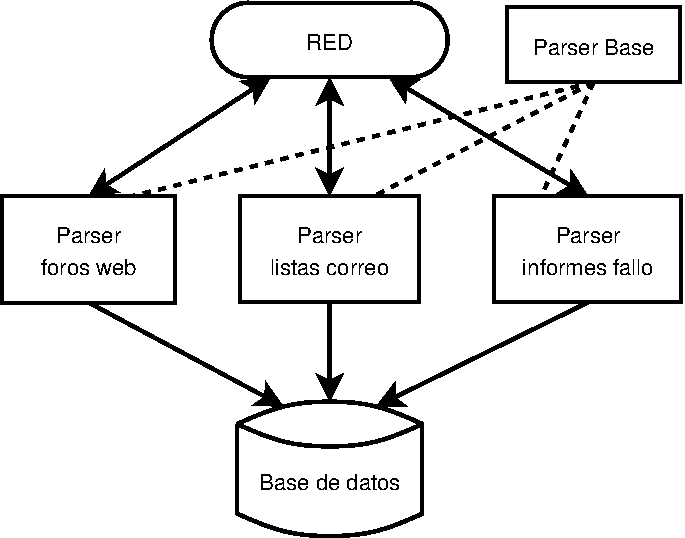
\includegraphics[width=9cm, keepaspectratio]{img/arquitectura}
%  \caption{Estructura del parser básico}
%  \label{fig:arquitectura}
%\end{figure}

%Si utilizas una base de datos, no te olvides de incluir también un diagrama de entidad-relación.


%%%%%%%%%%%%%%%%%%%%%%%%%%%%%%%%%%%%%%%%%%%%%%%%%%%%%%%%%%%%%%%%%%%%%%%%%%%%%%%%
%%%%%%%%%%%%%%%%%%%%%%%%%%%%%%%%%%%%%%%%%%%%%%%%%%%%%%%%%%%%%%%%%%%%%%%%%%%%%%%%
% RESULTS %
%%%%%%%%%%%%%%%%%%%%%%%%%%%%%%%%%%%%%%%%%%%%%%%%%%%%%%%%%%%%%%%%%%%%%%%%%%%%%%%%

\cleardoublepage
\chapter{Results}
\section{Introduction}
\label{sec:results-introduction}
On the previous chapter we saw in detail how the web application was developed step by step. On this chapter we are going to explain how this application works, how to use it and its functionality.

\section{User Guide}
\label{sec:results-user-guide}
On this section we are going to explain one by one how the web application's different features work. First we are going to begin with the "Visualizations" feature, we are going to explain each type of visualization and how to build them, then we are going to explain the "Dashboard" section and how to build dashboards from different visualizations.

\subsection{Visualizations}
\label{sec:results-visualizations}
The first view we are getting when we open the application, or clicking on the "eye" icon on the nav-bar, is the "Visualizations" section. We can see this view on Figure~\ref{fig:visualizations-section}.

From this view, if we open the "Saved Visualizations" by clicking on its bar (Figure~\ref{fig:saved-visualizations}),  we can either load a saved visualization or delete it by clicking on the trash icon.

Another option is to create a new visualization by opening the "Visualization Options" bar. To create a new visualization we must select an index about which we are going to calculate the available visualization types. This is shown on Figure~\ref{fig:visualization-options}.

Let's see how to create each of the visualization types.

\begin{figure}
  \centering
  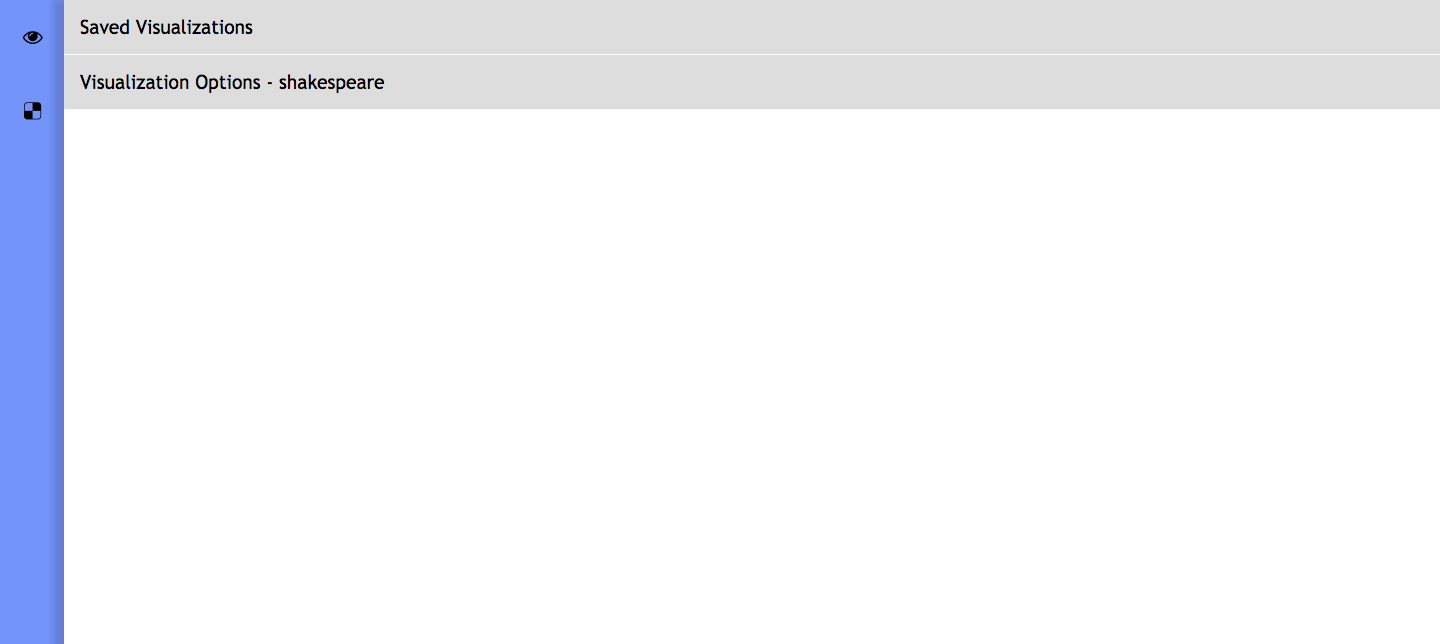
\includegraphics[width=13cm, keepaspectratio]{img/visualizations-section}
  \caption{Visualizations section}
  \label{fig:visualizations-section}
\end{figure}

\begin{figure}
  \centering
  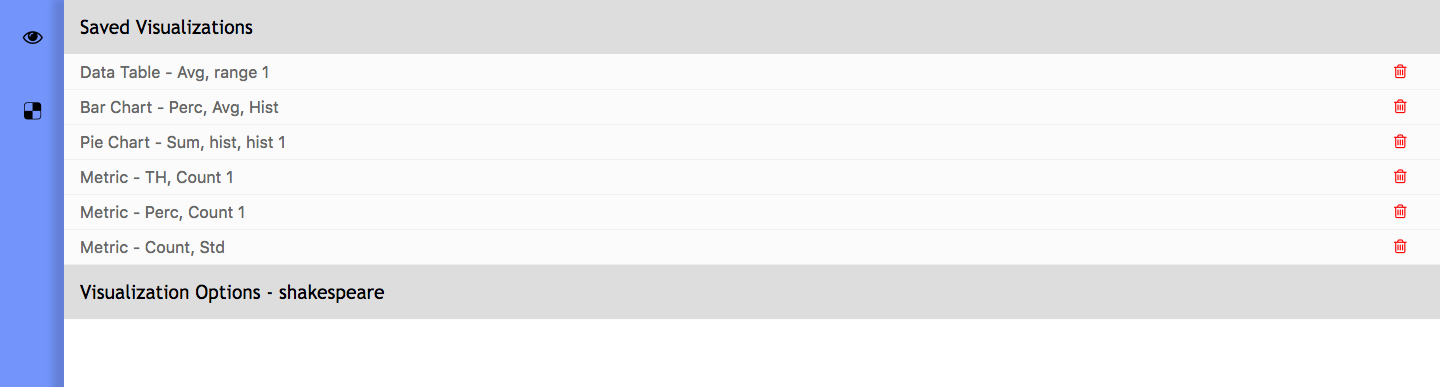
\includegraphics[width=13cm, keepaspectratio]{img/saved-visualizations.png}
  \caption{Saved Visualizations panel}
  \label{fig:saved-visualizations}
\end{figure}

\begin{figure}
  \centering
  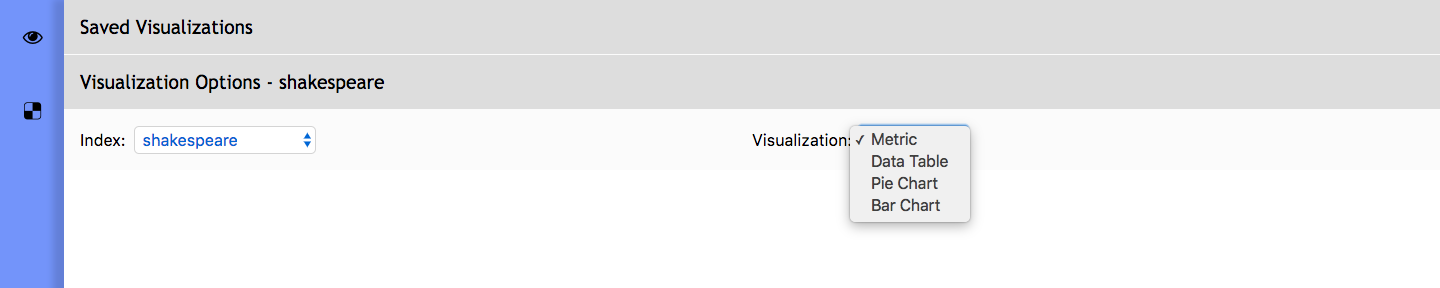
\includegraphics[width=13cm, keepaspectratio]{img/visualization-options.png}
  \caption{Visualization Options panel}
  \label{fig:visualization-options}
\end{figure}

\subsubsection{Metric Visualization}
\label{sec:metric-visualization}
A "Metric" visualization performs an operation over the index data an shows the result as a String, a Number or a collection of them. We can see an initial view of this "Metric Visualization" on Figure~\ref{fig:metric-visualization-initial-view}.

To add a metric operation to our visualization, we have to click on the "+" icon, this will add a "count" calculation over the selected index by default, and if we click the "play" icon we'll see the result on the screen (Figure~\ref{fig:metric-count-calcuation}).

\begin{figure}
  \centering
  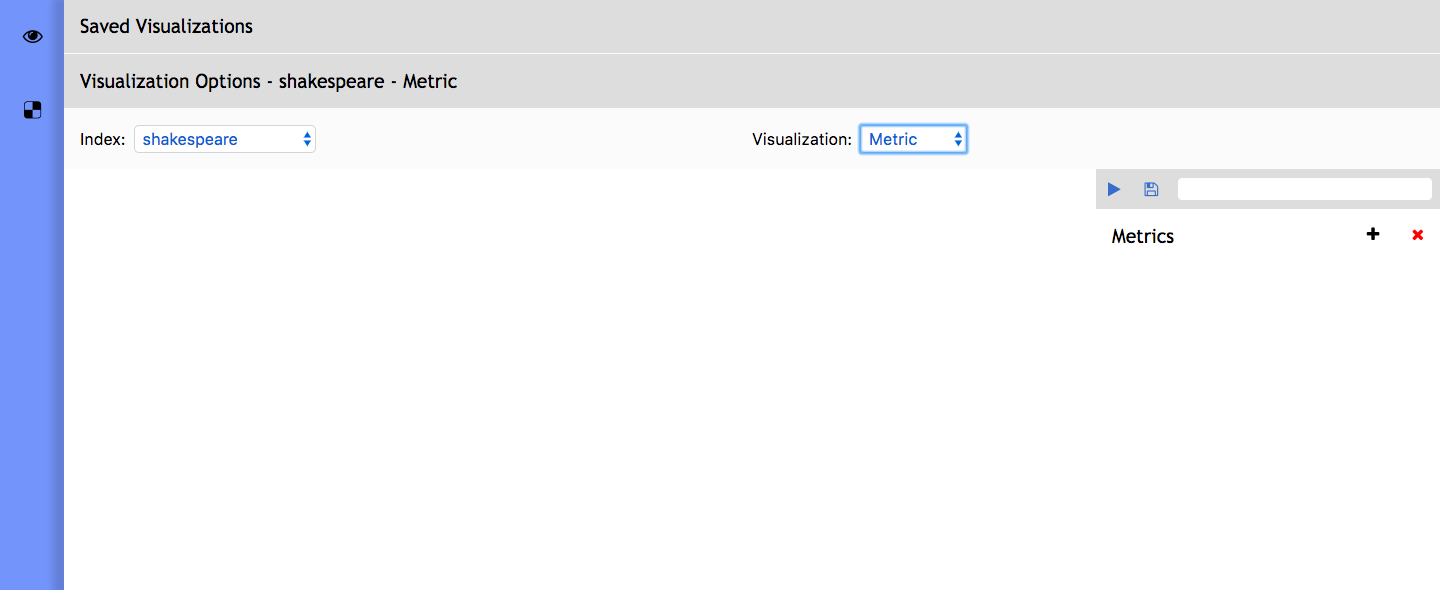
\includegraphics[width=13cm, keepaspectratio]{img/metric-visualization-initial-view.png}
  \caption{Initial view of a Metric Visualization}
  \label{fig:metric-visualization-initial-view}
\end{figure}

\begin{figure}
  \centering
  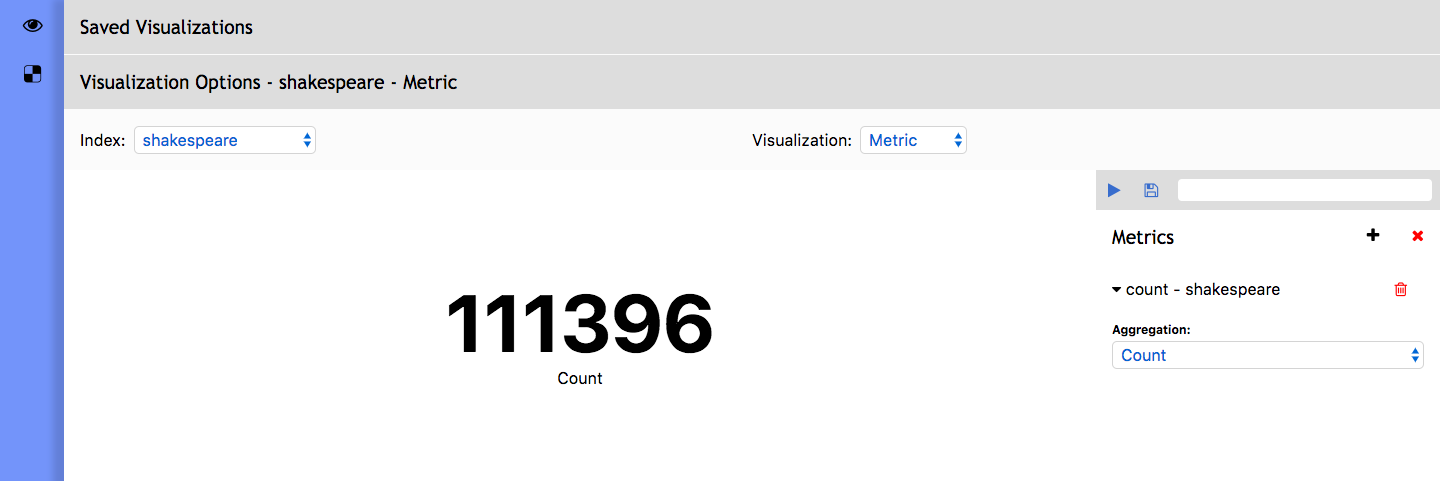
\includegraphics[width=13cm, keepaspectratio]{img/metric-count-calcuation.png}
  \caption{Metric "count" calculation}
  \label{fig:metric-count-calcuation}
\end{figure}

The operation description for each "aggregation" option is:
\begin{itemize}
    \item \textbf{Count}: Counts the exact number of documents for a given index (Figure~\ref{fig:metric-count-calcuation}).
    \item \textbf{Average}: Calculates the average for a given field of a documents collection for a given index. This field's type must be "number" (Figure~\ref{fig:metric-average-calcuation}).
    \item \textbf{Sum}: Calculates the summation over a documents collection for a given field and index. This field's type must be "number" (Figure~\ref{fig:metric-sum-calcuation}).
    \item \textbf{Min}: Calculates the minimum value for a given field of a documents collection for a given index. This field's type must be "number" (Figure~\ref{fig:metric-min-calcuation}).
    \item \textbf{Max}: Calculates the maximum value for a given field of a documents collection for a given index. This field's type must be "number" (Figure~\ref{fig:metric-max-calcuation}).
    \item \textbf{Median}: Calculates the median value for a given field of a documents collection for a given index. This field's type must be "number" (Figure~\ref{fig:metric-median-calcuation}).
    \item \textbf{Standard Deviation}: Calculates the standard deviation values for a given field of a documents collection for a given index. This field's type must be "number" (Figure~\ref{fig:metric-std-calcuation}).
    \item \textbf{Unique Count}: Calculates number of unique values for a given field of a documents collection for a given index. This field's type must be "number" (Figure~\ref{fig:metric-unique-calcuation}).
    \item \textbf{Percentiles}: Calculates a multi-values percentiles result for a given field of a documents collection for a given index and for a given list of percentiles. This field's type must be "number" (Figure~\ref{fig:metric-percentiles-calcuation}).
    \item \textbf{Percentile Ranks}: Calculates a multi-values percentiles result for a given field of a documents collection for a given index and for a given list of percentiles. This field's type must be "number". Percentile ranks show the percentage of documents which selected field's value is below certain value (Figure~\ref{fig:metric-ranks-calcuation}).
    \item \textbf{Top Hits}: This aggregation is very different from the others. Top Hits keeps track of the top matching documents depending on the selected options and fields. We have to select multiple options in order to perform the aggregation calculation (Figure~\ref{fig:metric-top-calcuation}). These fields are:
    \begin{itemize}
        \item \textbf{Field}: This is the same as with the other aggregations, it indicates the document field over which we are going to perform the request.
        \item \textbf{Aggregate With}: This indicates the way we are going to process the received hits, such as "summation", "maximum", "minimum", "average" or "concatenation". Except for the last type, all must be with a "number" type field.
        \item \textbf{Size}: This indicates the maximum number of documents or hits we are going to receive on the response.
        \item \textbf{Sort On}: This, again, is a document field. This field affects to the documents or hits we are going to receive in the way that these documents are going to be sorted by this field. If this field is a "number", the documents will be sorted "numerically", and if the field is a "string", the documents will be sorted alphabetically.
        \item \textbf{Order}: This indicates how the documents will be sorted, i.e. ascending or descending.
    \end{itemize}
\end{itemize}

\begin{figure}
  \centering
  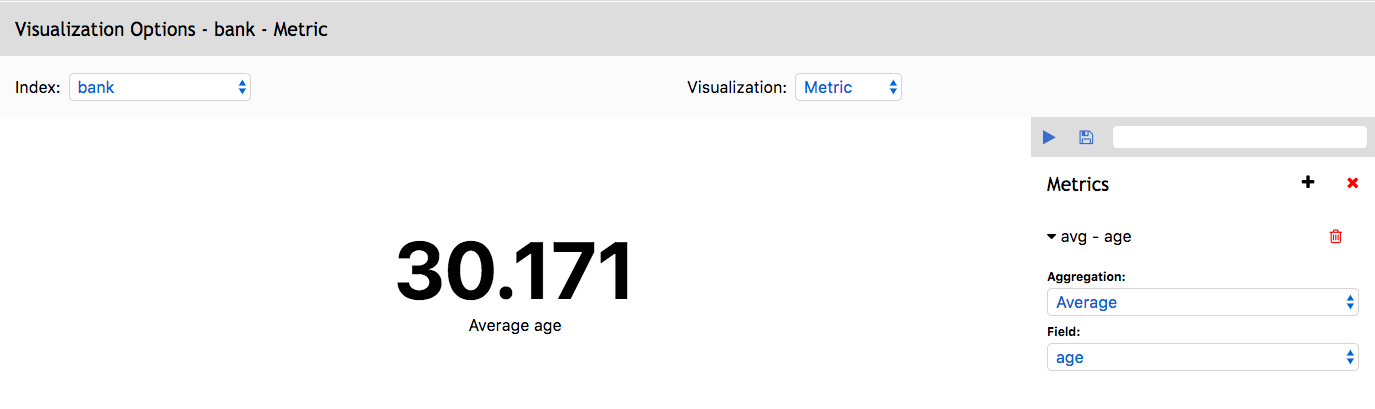
\includegraphics[width=13cm, keepaspectratio]{img/metric-average-calculation.png}
  \caption{Metric "average" calculation}
  \label{fig:metric-average-calcuation}
\end{figure}

\begin{figure}
  \centering
  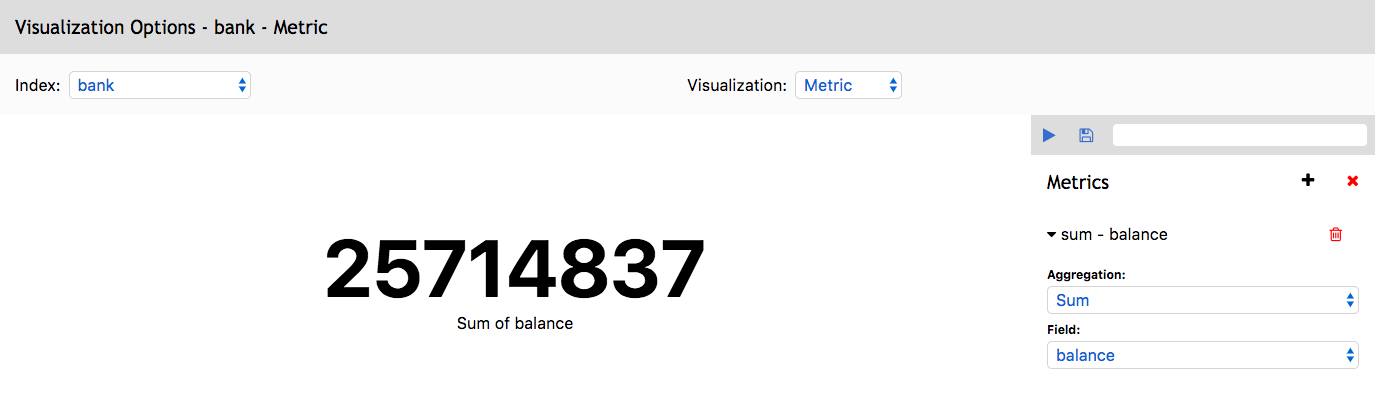
\includegraphics[width=13cm, keepaspectratio]{img/metric-sum-calculation.png}
  \caption{Metric "sum" calculation}
  \label{fig:metric-sum-calcuation}
\end{figure}

\begin{figure}
  \centering
  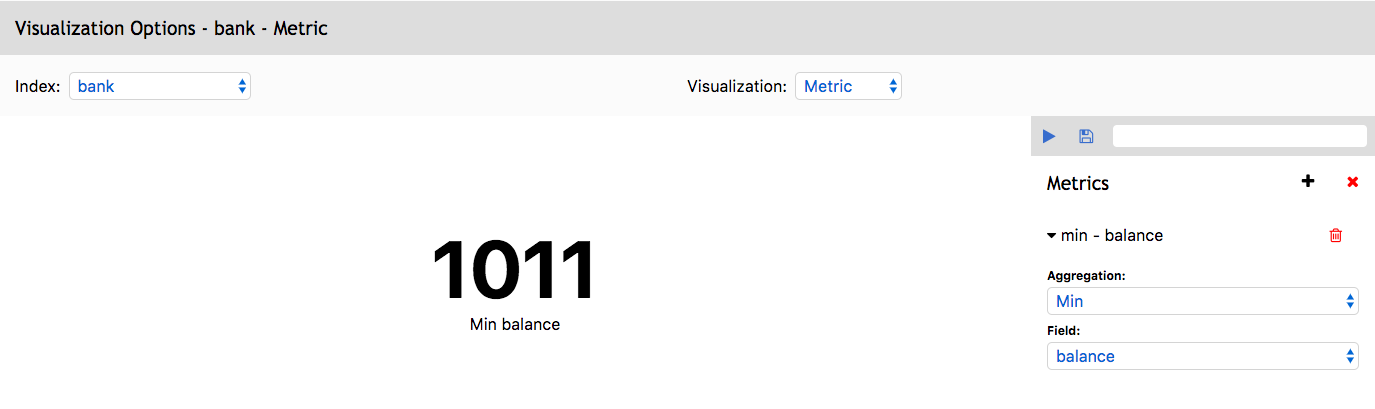
\includegraphics[width=13cm, keepaspectratio]{img/metric-min-calculation.png}
  \caption{Metric "min" calculation}
  \label{fig:metric-min-calcuation}
\end{figure}

\begin{figure}
  \centering
  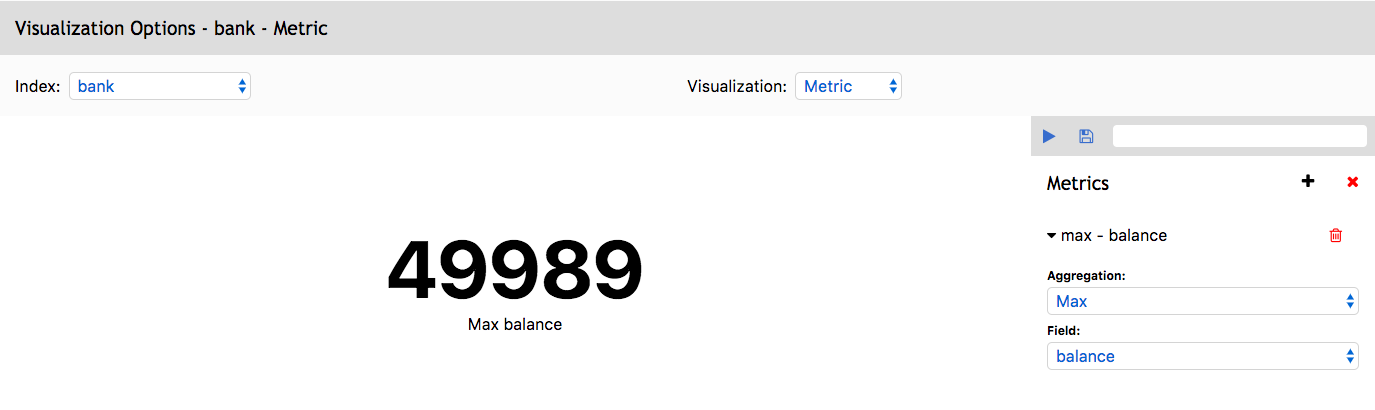
\includegraphics[width=13cm, keepaspectratio]{img/metric-max-calculation.png}
  \caption{Metric "max" calculation}
  \label{fig:metric-max-calcuation}
\end{figure}

\begin{figure}
  \centering
  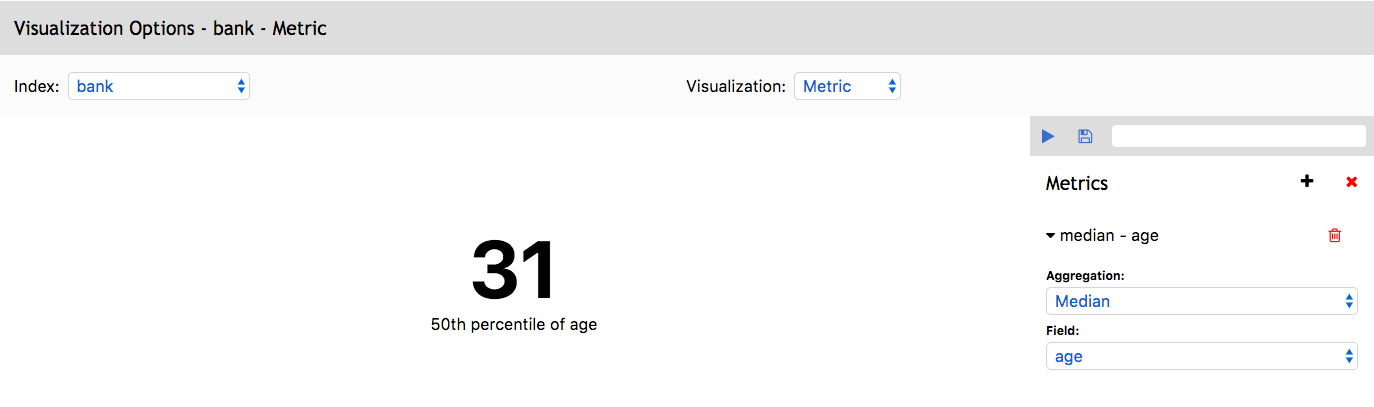
\includegraphics[width=13cm, keepaspectratio]{img/metric-median-calculation.png}
  \caption{Metric "median" calculation}
  \label{fig:metric-median-calcuation}
\end{figure}

\begin{figure}
  \centering
  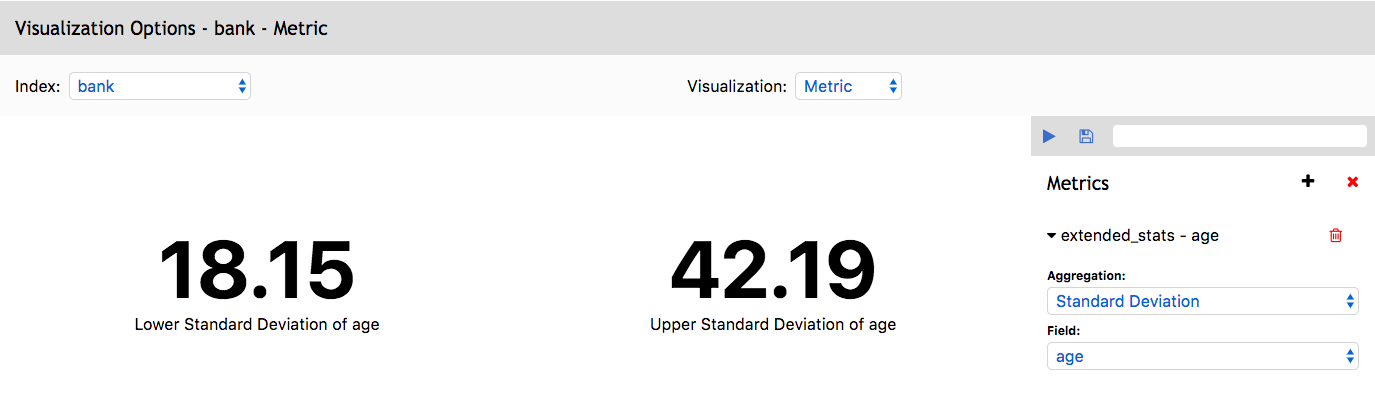
\includegraphics[width=13cm, keepaspectratio]{img/metric-std-calculation.png}
  \caption{Metric "standard deviation" calculation}
  \label{fig:metric-std-calcuation}
\end{figure}

\begin{figure}
  \centering
  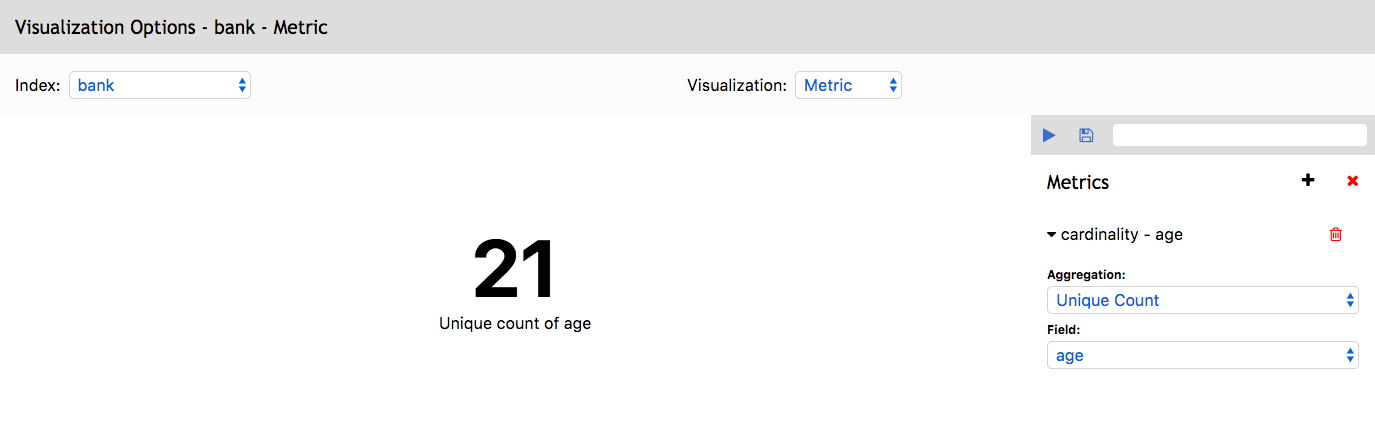
\includegraphics[width=13cm, keepaspectratio]{img/metric-unique-calculation.png}
  \caption{Metric "unique count" calculation}
  \label{fig:metric-unique-calcuation}
\end{figure}

\begin{figure}
  \centering
  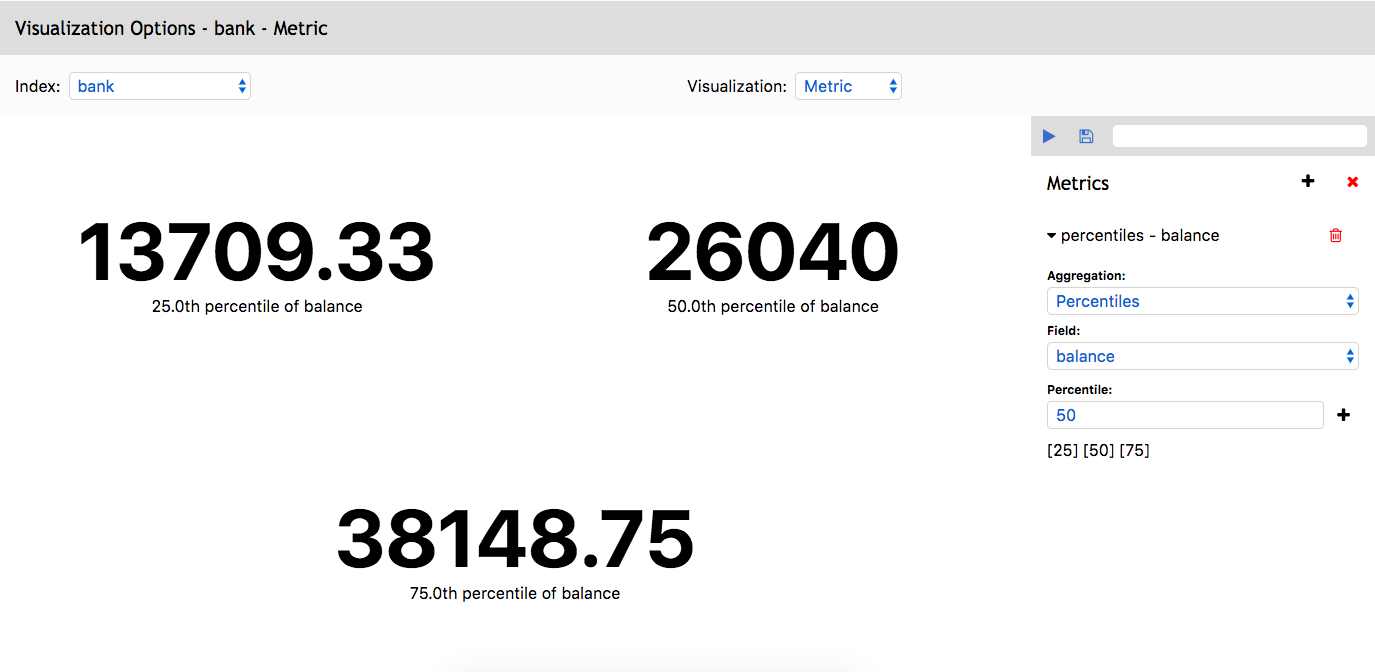
\includegraphics[width=13cm, keepaspectratio]{img/metric-percentiles-calculation.png}
  \caption{Metric "percentiles" calculation}
  \label{fig:metric-percentiles-calcuation}
\end{figure}

\begin{figure}
  \centering
  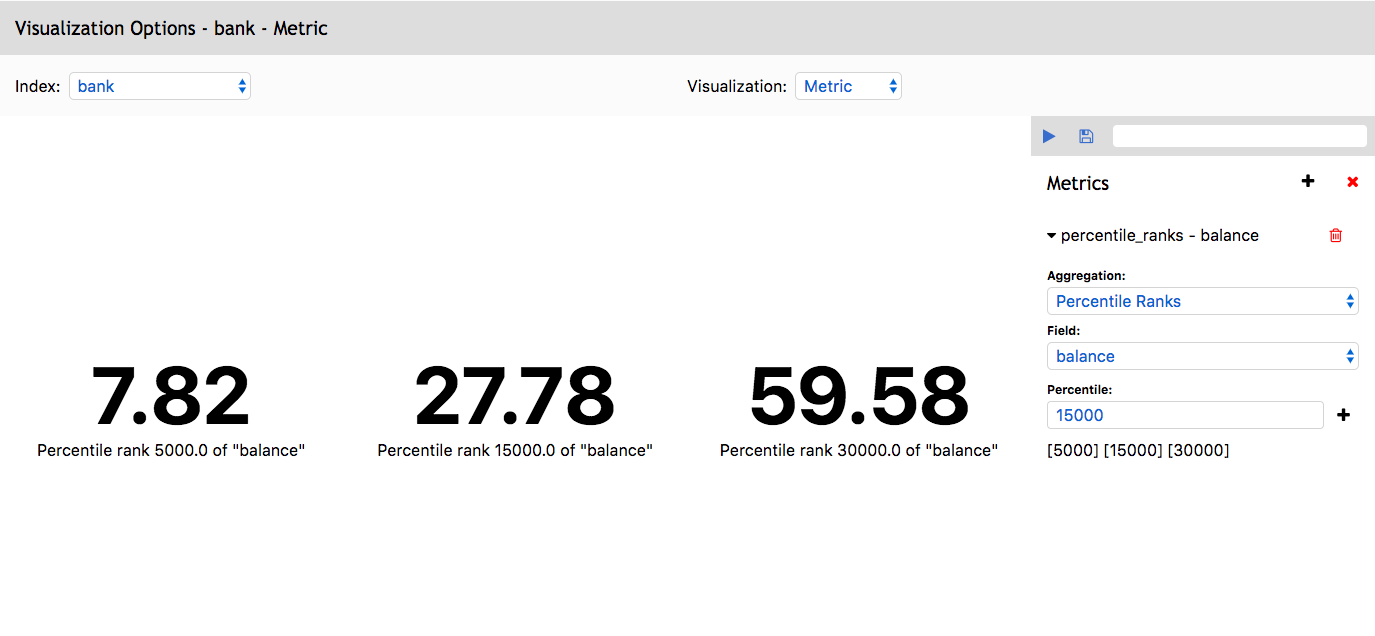
\includegraphics[width=13cm, keepaspectratio]{img/metric-ranks-calculation.png}
  \caption{Metric "percentile ranks" calculation}
  \label{fig:metric-ranks-calcuation}
\end{figure}

\begin{figure}
  \centering
  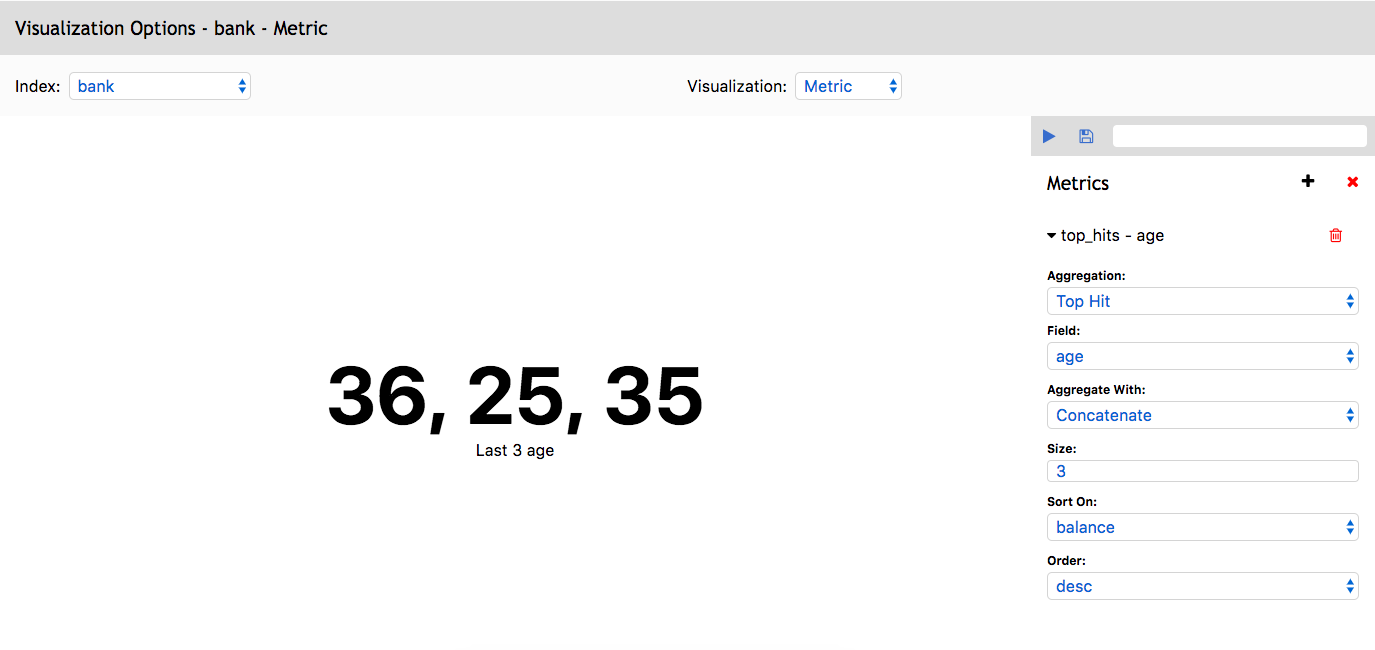
\includegraphics[width=13cm, keepaspectratio]{img/metric-top-calculation.png}
  \caption{Metric "top hits" calculation}
  \label{fig:metric-top-calcuation}
\end{figure}

\subsubsection{Data Table Visualization}
\label{sec:data-table-visualization}
A "Data Table" visualization performs an operation over the index data and shows the result as a table. We can see an initial view of this "Data Table Visualization" on Figure~\ref{fig:data-table-initial-view}.
\begin{figure}
  \centering
  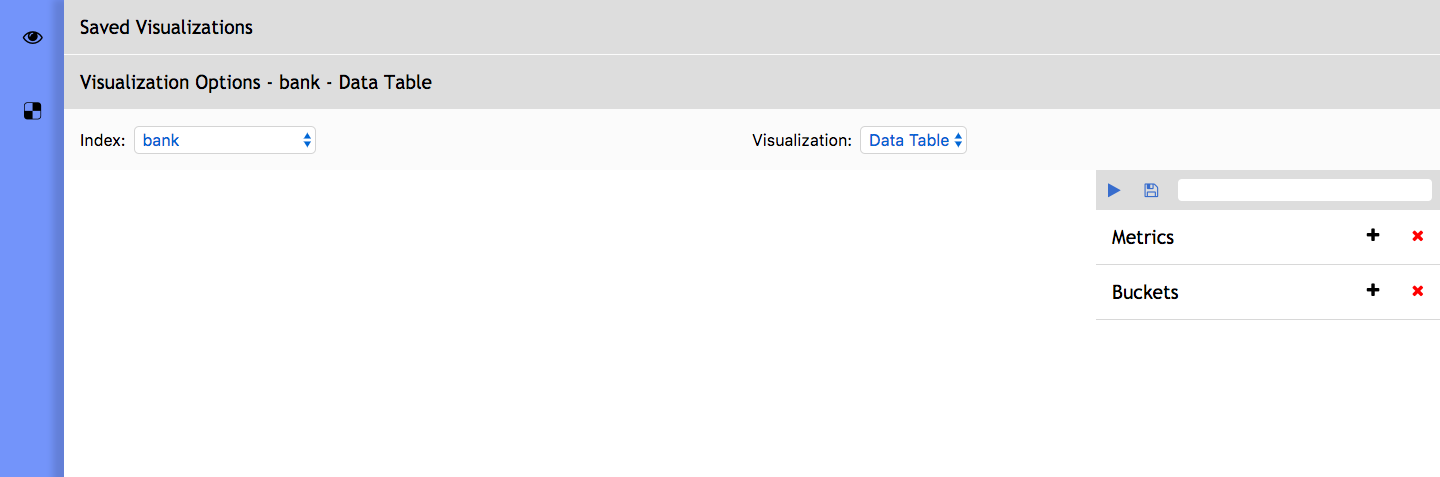
\includegraphics[width=13cm, keepaspectratio]{img/data-table-initial-view.png}
  \caption{Data Table visualization initial view}
  \label{fig:data-table-initial-view}
\end{figure}

As we can see, we have a new element on the configuration panel, "Buckets". This bucket aggregations defines a rule to create buckets of documents when making requests to Elasticsearch. Now, the metrics will be performed over this buckets of documents.

We have two types of bucket aggregations:
\begin{itemize}
    \item \textbf{Histogram}: This aggregation builds interval buckets of documents for a given numeric field and numeric interval value (Figure~\ref{fig:data-table-histogram-calculation-view}).
    \item \textbf{Range}: This aggregation builds range buckets of documents for a given numeric field and a collection of numeric ranges (Figure~\ref{fig:data-table-range-calculation}).
\end{itemize}

The table will have as many columns as metric results plus the number of buckets. And it will have as many rows as received hits over all buckets.

The table allows any number of metrics and any number of buckets. If we have more than one bucket, the bucket results will be created recursively (Figure~\ref{fig:data-table-multiaggregation-calculation}).

\begin{figure}
  \centering
  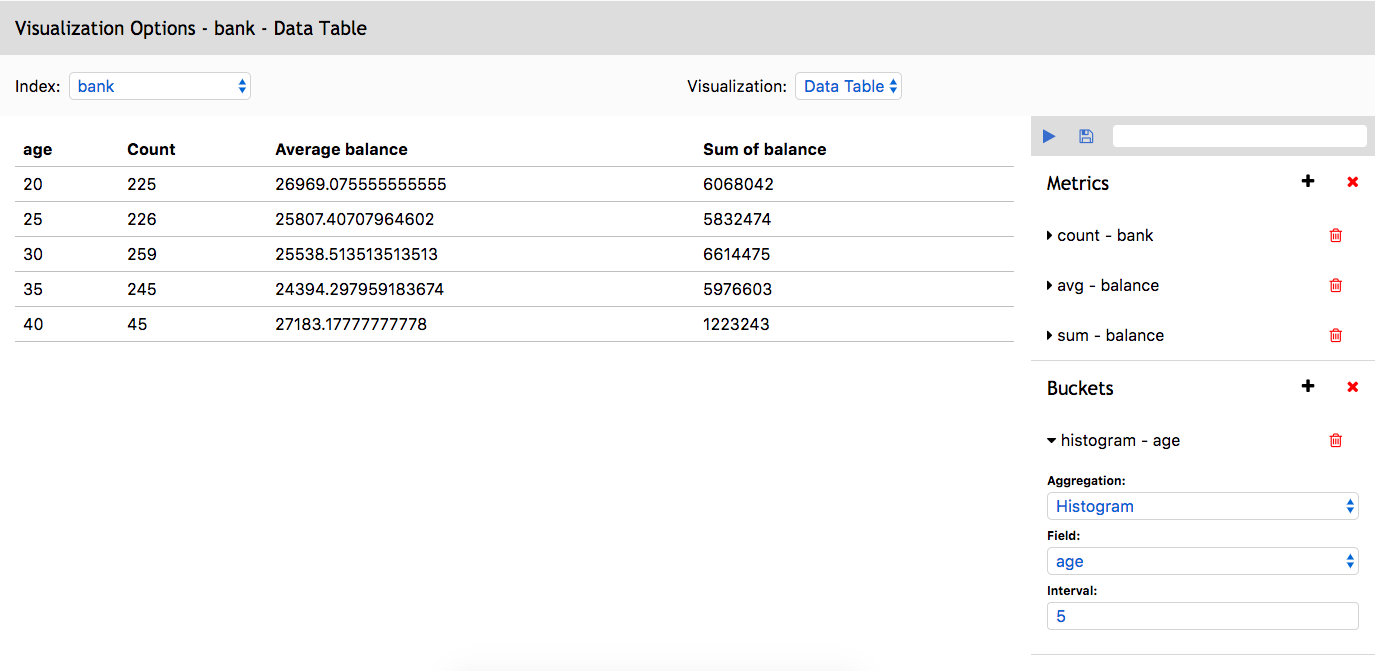
\includegraphics[width=13cm, keepaspectratio]{img/data-table-histogram-calculation.png}
  \caption{Data Table histogram example.}
  \label{fig:data-table-histogram-calculation-view}
\end{figure}

\begin{figure}
  \centering
  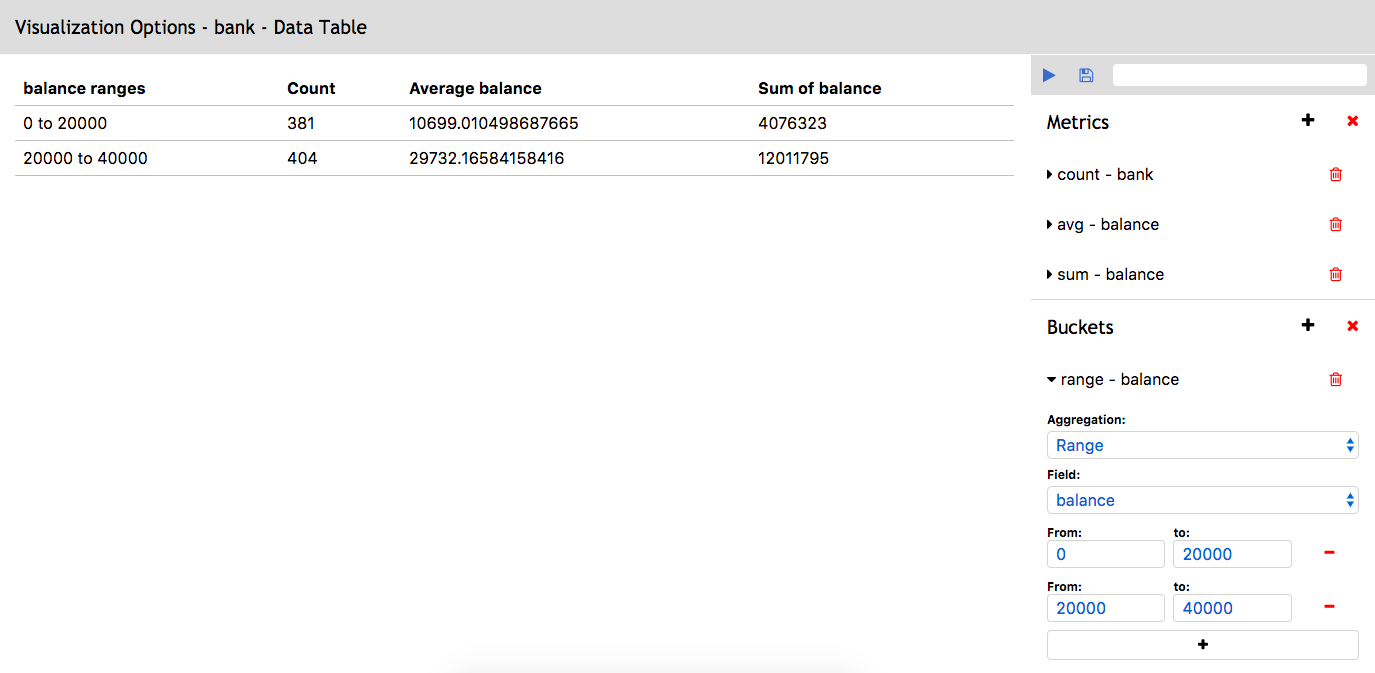
\includegraphics[width=13cm, keepaspectratio]{img/data-table-range-calculation.png}
  \caption{Data Table range example.}
  \label{fig:data-table-range-calculation}
\end{figure}

\begin{figure}
  \centering
  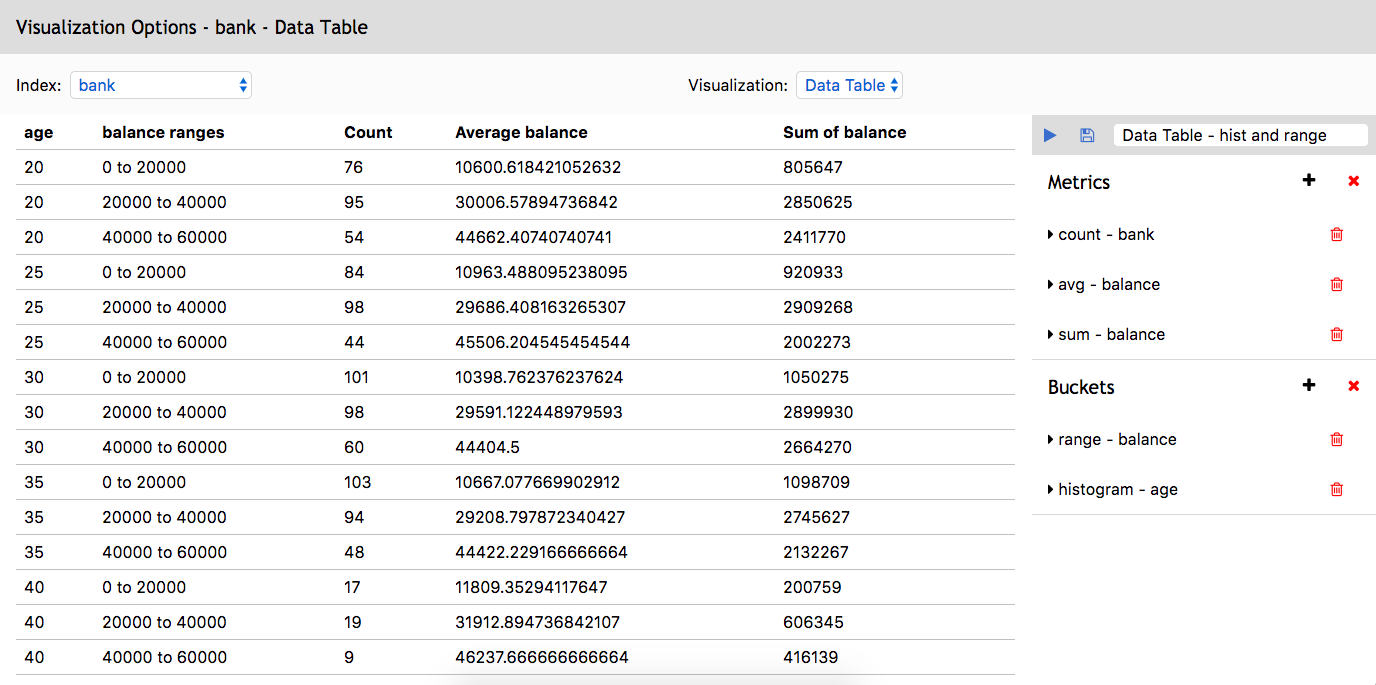
\includegraphics[width=13cm, keepaspectratio]{img/data-table-multiaggregation-calculation.png}
  \caption{Data Table multiple buckets example.}
  \label{fig:data-table-multiaggregation-calculation}
\end{figure}


\subsubsection{Pie Chart Visualization}
\label{sec:pie-chart-visualization}
A "Pie Chart" visualization performs an operation over the index data an shows the result as a pie chart. The initial view is the same as the "Data Table" visualization's.

To create a "Pie Chart" visualization we have to create one or more buckets and one metric maximum. We will have as many levels or rings on our "Pie Chart" as the number of buckets. For the metrics creation, it only works with "Count", "Sum", "Unique Count" and "Top Hit" aggregations.

This chart introduces the label \textit{tooltip} that shows up when hovering over a "Pie Chart" slice. Because we have different levels, the \textit{tooltip} shows a table whose rows appertain to each bucket aggregation.

An example of a "Pie Chart" visualization is shown on Figure~\ref{fig:pie-chart-calculation}.

\begin{figure}
  \centering
  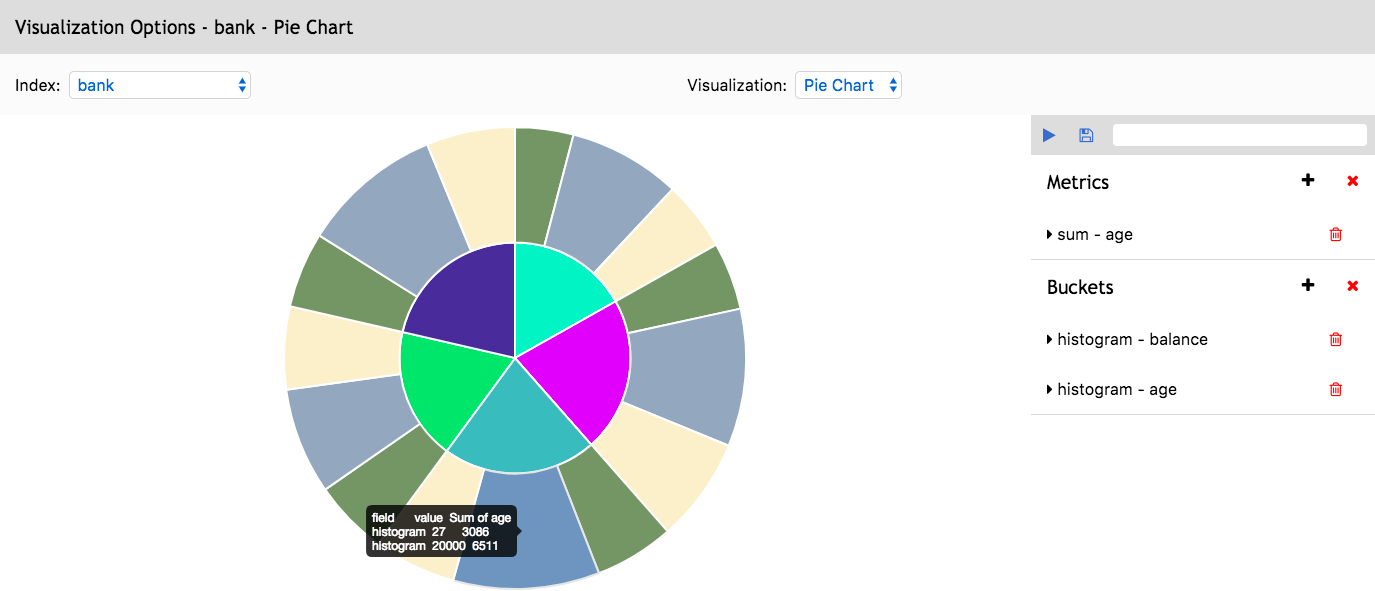
\includegraphics[width=16cm, keepaspectratio]{img/pie-chart-calculation.png}
  \caption{Pie Chart example.}
  \label{fig:pie-chart-calculation}
\end{figure}

\subsubsection{Bar Chart Visualization}
\label{sec:bar-chart-visualization}
A "Bar Chart" visualization performs an operation over the index data an shows the result as a bar chart. The initial view is the same as the "Data Table" visualization's.

To create a "Bar Chart" visualization we have to create one or more metrics and one bucket maximum. We will have as many bars as buckets of documents. The metric results will stack on the bars.

This chart has a label \textit{tooltip} as the "Pie chart" visualization, but this time the \textit{tooltip} shows the metric field value for a specific bucket.

An example of a "Bar Chart" visualization is shown on Figure~\ref{fig:bar-chart-calculation}.
\begin{figure}
  \centering
  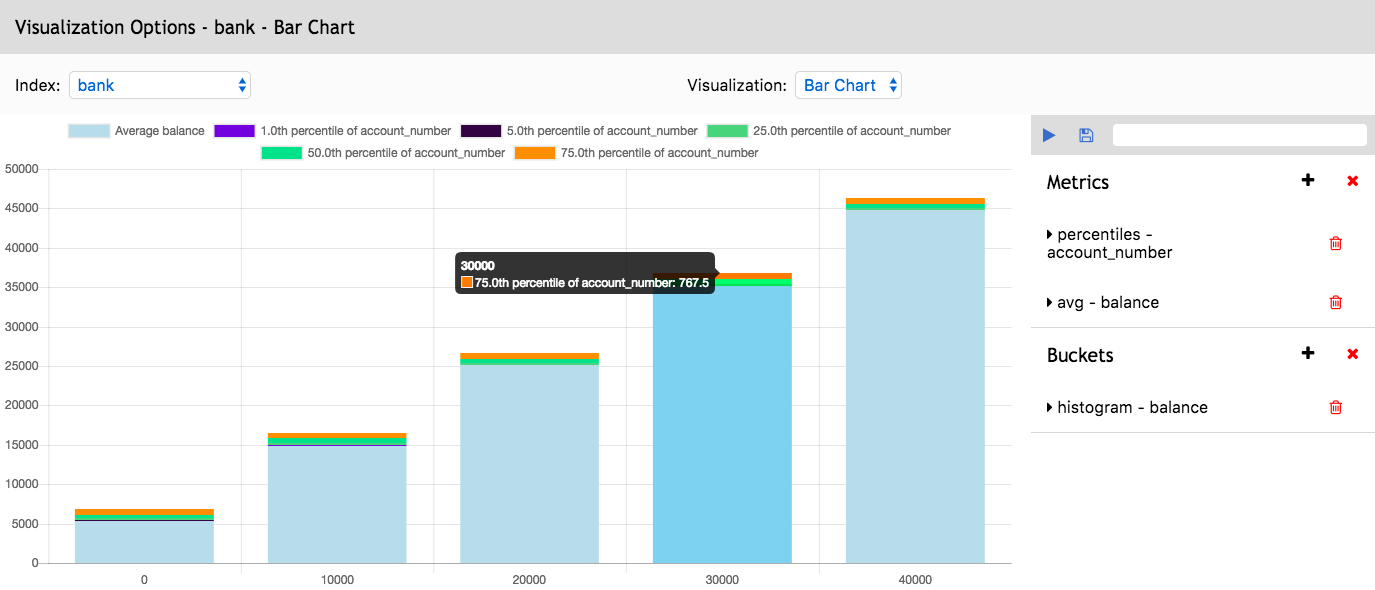
\includegraphics[width=16cm, keepaspectratio]{img/bar-chart-calculation.png}
  \caption{Bar Chart example.}
  \label{fig:bar-chart-calculation}
\end{figure}

This chart introduces the chart \textit{legend}. The legend specifies which color appertains to each metric result. In addition, this legend allows to filter some metric results disabling them by clicking on them, an example of the same "Bar Chart" with a filtered result is shown on Figure~\ref{fig:bar-chart-lengend-filter-example}.
\begin{figure}
  \centering
  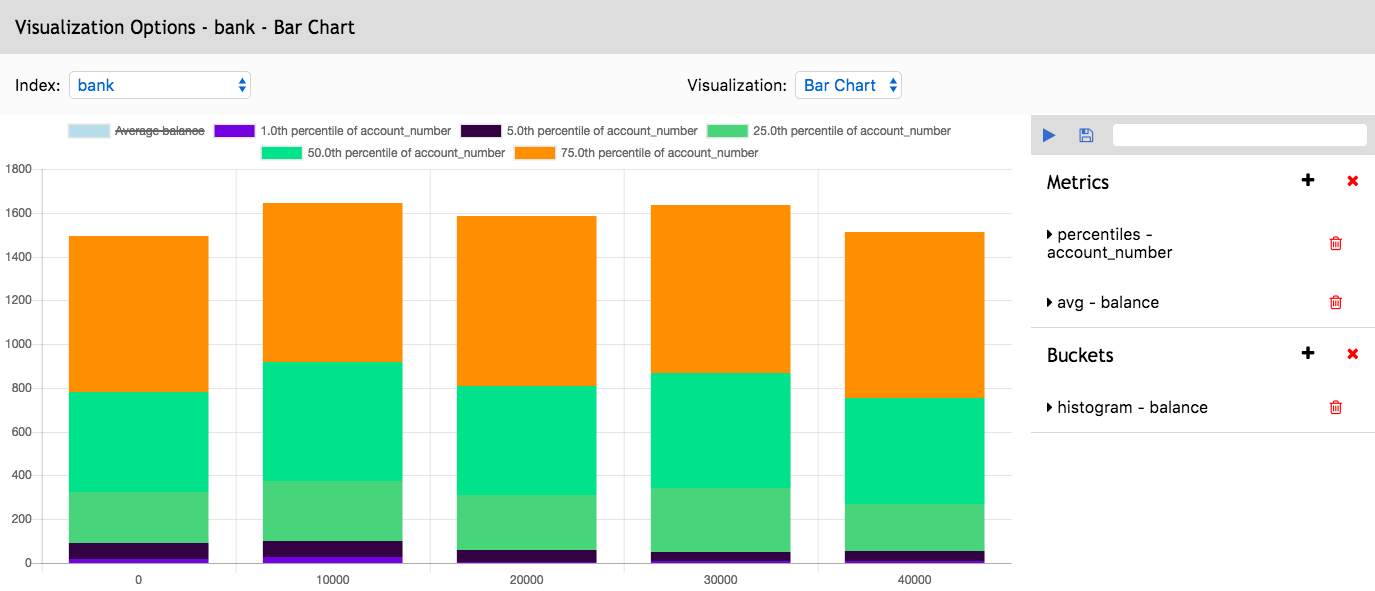
\includegraphics[width=16cm, keepaspectratio]{img/bar-chart-lengend-filter-example.png}
  \caption{Filtered Bar Chart example.}
  \label{fig:bar-chart-lengend-filter-example}
\end{figure}

\subsubsection{Saving Visualizations}
\label{sec:saving-visualizations}
We finish this section by explaining how saving visualizations works. To save a visualization we only have to write a visualization title, on the input at the top of our "metrics and buckets" panel, and click on the "floppy disk" icon. If we want to edit a visualization, after loading it from the "Saved Visualizations" panel and modifying it, we only have to save it with the same title in order to overwrite it.


\subsection{Dashboards}
\label{sec:results-dashboards}
Dashboard is the application's second and last section. It can be accessed by clicking the "board" icon on the nav-bar. On Figure~\ref{fig:dashboards-initial-view} we can see the initial vie of this section.
\begin{figure}
  \centering
  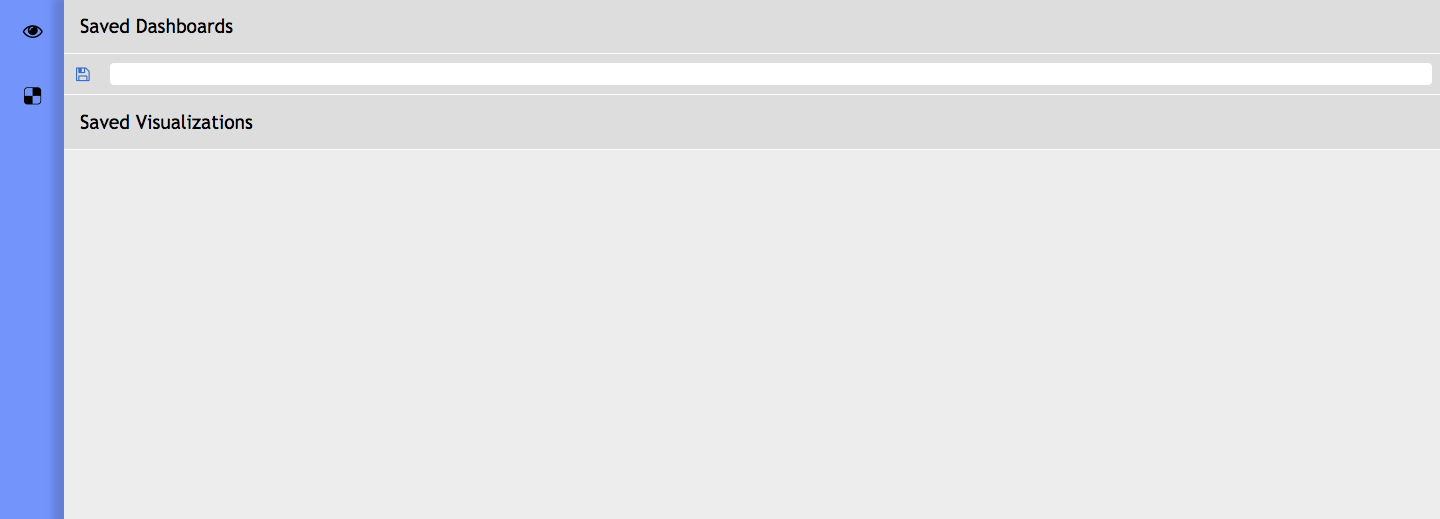
\includegraphics[width=16cm, keepaspectratio]{img/dashboards-initial-view.png}
  \caption{Dashboard section.}
  \label{fig:dashboards-initial-view}
\end{figure}

On this section we can create, delete and edit dashboards. All dashboards are created from previously saved visualizations.

To load a saved dashboard we just have to select one from the "Saved Dashboards" section, and to delete a dashboard we only have to click its "trash" icon.

To create a new dashboard, we have to open the "Saved Visualizations" section and begin to select each saved visualization we want to add into our new dashboard. We can add multiple times the same visualization.

On Figure~\ref{fig:dashboards-initial-view} we can see how it looks a dashboard with visualizations.
\begin{figure}
  \centering
  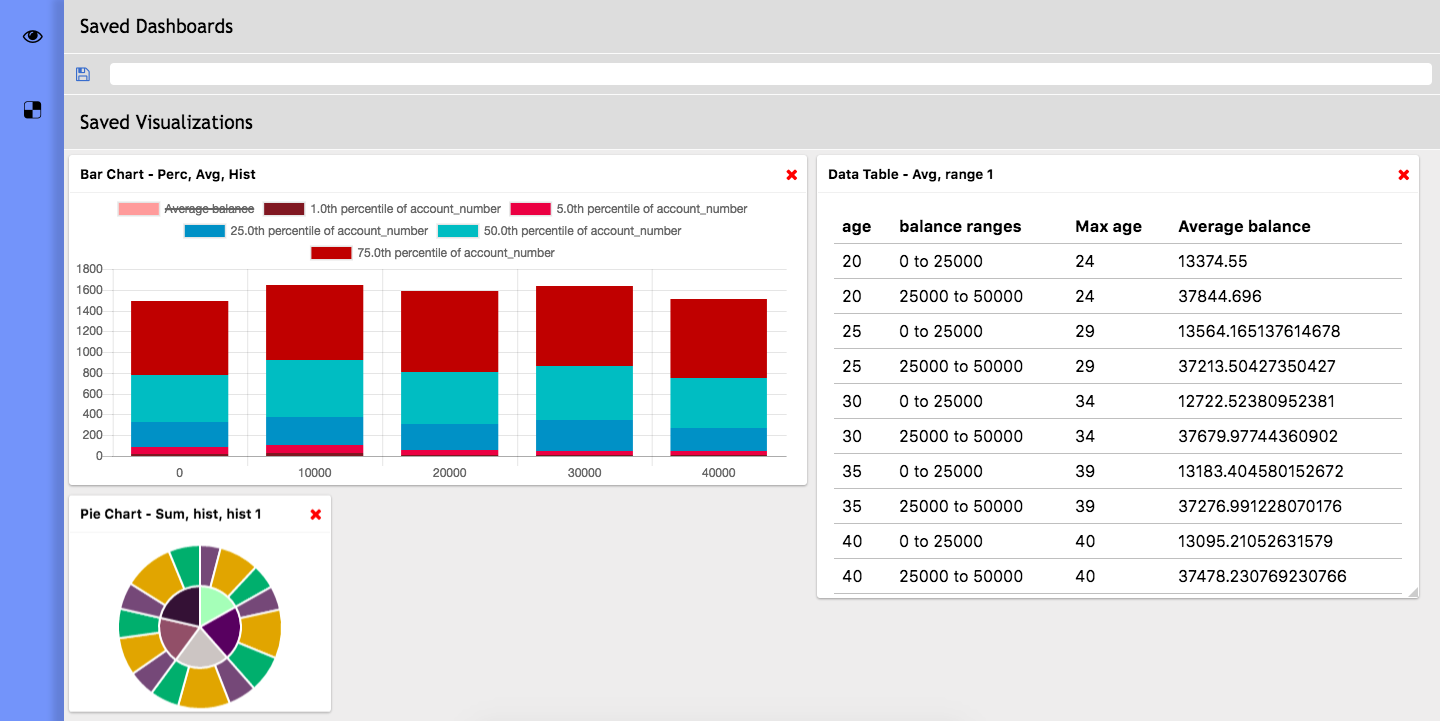
\includegraphics[width=16cm, keepaspectratio]{img/dashboard-example.png}
  \caption{Dashboard example.}
  \label{fig:dashboard-example}
\end{figure}

To edit a dashboard we can:
\begin{itemize}
    \item Remove a visualization from the dashboard clicking on the "x" icon on the top right corner.
    \item Add more visualizations.
    \item Move visualizations by clicking on the visualization title, dragging and dropping the visualization on the desired position.
\end{itemize}

The saving process is the same as the "Visualizations" saving process.

%En este capítulo se incluyen los resultados de tu trabajo fin de grado.

%Si es una herramienta de análisis lo que has realizado, aquí puedes poner ejemplos de haberla utilizado para que se vea su utilidad.


%%%%%%%%%%%%%%%%%%%%%%%%%%%%%%%%%%%%%%%%%%%%%%%%%%%%%%%%%%%%%%%%%%%%%%%%%%%%%%%%
%%%%%%%%%%%%%%%%%%%%%%%%%%%%%%%%%%%%%%%%%%%%%%%%%%%%%%%%%%%%%%%%%%%%%%%%%%%%%%%%
% CONCLUSIONES %
%%%%%%%%%%%%%%%%%%%%%%%%%%%%%%%%%%%%%%%%%%%%%%%%%%%%%%%%%%%%%%%%%%%%%%%%%%%%%%%%

\cleardoublepage
\chapter{Conclusions}
\label{chap:conclusions}

\section{Objectives achievement}
\label{sec:objectives-achievement}

If we look back to the main objectives we'll see that they have been fulfilled. We have developed an application using Elasticsearch and its API.

We were able to implement a tool that allows us to create a different types of visualizations such as "Metrics", "Data Tables", "Pie Charts" and "Bar Charts". This application allow us to save this visualizations, load them from the Elasticsearch database, modify them and delete them from Elasticsearch.

In addition, this application has another section where we can create and design our personalized dashboards of saved visualizations. This dashboards can be stored on the Elasticsearch database in order to load them later and modify them or delete them.

One of this project's objective was learning how to use modern technologies of framework based construction in javascript, or in this case its superset Typescript, such as Angular. Effectively, this application has been developed with Angular and we had taken advantage from several of its features, which saved us working time when developing the application. In addition, this features have allowed us to develop a more flexible application such us:
\begin{itemize}
    \item \textit{Routing}: To make the application navigation for the different structure sections, making easily a SPA.
    \item \textit{Injection}: Allowing as to integrate and reuse different modules in a simple way, and saving us working time.
    \item \textit{Services} - Standard use: To make isolated code where we interact with the database to retrieve or manage data from the database, making a cleaner and more readable code.
    \item \textit{Services} - Custom use: To communicate between different components, fixing the component variable dependency synchronization issues due to the Angular "livecycle" hook.
    \item \textit{Components}: To make a well structured code where each component had its own functionality.
\end{itemize}

In addition, we had another objective for this project, this is finding out how could we integrate different visualization libraries with Angular such as \textit{ChartJS}. We found that Angular has different options to integrate external libraries such as the common way with the library CDN, or importing the library module with NPM, but this module required to have a "typings" (Typescript) file with the variable types declaration in order to have it work in our project. In this case we used both techniques due to missing "typings" files for some libraries we used, or due to limitations by using the second option.

Thus, we achieved an HTML5 application development, we worked with a no-SQL database such as Elasticsearch, we used already implemented components to interact with it, so we used an API which allowed us to have a dynamic access to the data. We use the data writing in order to have a data persistence on whatever the user creates, thus, the user can save its progress whenever the user wants and recover the work later, in the same state the user left it. In addition, the application is very flexible, it does not require a defined data but it works with any type of data since the user interface allows us to choose the data, from the stored data on the database.

With this, we have built visualizations using external libraries, and we have built too, a dashboard structure that allowed us to combine visualizations in the same panel. In addition, in an introspective way, in real time we read the data from the database, and we use this data to build the buckets and the metrics, thus, the user can choose to show another type of visualization if the data changes. So we are not restricting to a concrete type of data on the back-end.

As we said, from the data, we can build or define groups of data (buckets), or we can build or define how those visualizations are summarized (metrics). And we have several ways to summarize them and several ways to group them, each one of them with different types of visualizations.

All this works over javascript on the web browser, without having to install anything else and without any specific API. This is because we work directly with the Elasticsearch API on the server side, everything else are libraries that we've integrated within our application. So, this application is a SPA which is responsive and works both on desktop and on tablets, thanks to Angular and Flexbox.

Finally, we have deployed too, a web site where we try to explain this project and appraise its application\footnote{\url{https://islimane.github.io/Angular-ElasticSearch-Dashboard_Interface/}}.

%Esta sección es la sección espejo de las dos primeras del capítulo de objetivos, donde se planteaba el objetivo general y se elaboraban los específicos.

%Es aquí donde hay que debatir qué se ha conseguido y qué no.
%Cuando algo no se ha conseguido, se ha de justificar, en términos de qué problemas se han encontrado y qué medidas se han tomado para mitigar esos problemas.


\section{Application of lessons learned}
\label{sec:application-of-lessons-learned}
During the course of the degree, a lot of knowledge has been acquired but not all this knowledge has been applied or necessary to develop this project. There are some subjects that have related content with this project such as "Telematic Applications Development", "Information Systems Engineering", "Programming Fundamentals", "Telematic Systems Engineering" or "Telematic Applications Systems". All this subjects has lessons that have been applied to this project such as data structures, javascript language and javascript libraries, web styling (css), html, version control or object classes.

%Aquí viene lo que has aprendido durante el Grado/Máster y que has aplicado en el TFG/TFM. Una buena idea es poner las asignaturas más relacionadas y comentar en un párrafo los conocimientos y habilidades puestos en práctica.

%\begin{enumerate}
%  \item a
%  \item b
%\end{enumerate}


\section{Learned Lessons}
\label{sec:learned-lessons}

On this project we've used a lot of tools and technologies that have not been tough during the degree course. During the project development I have learned or improved the following skills:
\begin{itemize}
    \item I've learned how to create and develop a project with Angular from scratch, how to retrieve data asynchronously with services, create a routing navigation for the web application, and a lot of Angular technologies or features.
    \item I've learned how to use the Elasticsearch API rest to retrieve data, create indexes, types and mappings, and to delete and overwrite data.
    \item I've learned how to use Flexbox to style and design a web application.
    \item I've learned how to use SASS to style a web application making the code more readable and simplified.
    \item I've learned how to use Typescript as a front-end programming language to develop a web application.
    \item I've learned how to create and modify Kibana visualizations and dashboards.
    \item I've learned how to manage a web application project with Webpack, installing and updating packages.
    \item I've improved my jQuery skills.
\end{itemize}

%Aquí viene lo que has aprendido en el Trabajo Fin de Grado/Máster.

%\begin{enumerate}
%  \item a
%  \item b
%\end{enumerate}


\section{Future Work}
\label{sec:future-work}
This project have a lot of possibilities when thinking on how to develop more features. These are a few of the future works:
\begin{itemize}
    \item Include more types of visualizations such as line charts, heat maps or even 3D charts.
    \item Include more bucket types such as date histograms.
    \item Allow to make real-time queries.
    \item Allow to change between visualizations sharing compatible data.
    \item Implement user accounts and log-in.
\end{itemize}



%Ningún software se termina, así que aquí vienen ideas y funcionalidades que estaría bien tener implementadas en el futuro.

%Es un apartado que sirve para dar ideas de cara a futuros TFGs/TFMs.


%%%%%%%%%%%%%%%%%%%%%%%%%%%%%%%%%%%%%%%%%%%%%%%%%%%%%%%%%%%%%%%%%%%%%%%%%%%%%%%%
%%%%%%%%%%%%%%%%%%%%%%%%%%%%%%%%%%%%%%%%%%%%%%%%%%%%%%%%%%%%%%%%%%%%%%%%%%%%%%%%
% APÉNDICE(S) %
%%%%%%%%%%%%%%%%%%%%%%%%%%%%%%%%%%%%%%%%%%%%%%%%%%%%%%%%%%%%%%%%%%%%%%%%%%%%%%%%

\cleardoublepage
%\appendix
%\chapter{Manual de usuario}
%\label{app:manual}


%%%%%%%%%%%%%%%%%%%%%%%%%%%%%%%%%%%%%%%%%%%%%%%%%%%%%%%%%%%%%%%%%%%%%%%%%%%%%%%%
%%%%%%%%%%%%%%%%%%%%%%%%%%%%%%%%%%%%%%%%%%%%%%%%%%%%%%%%%%%%%%%%%%%%%%%%%%%%%%%%
% BIBLIOGRAFIA %
%%%%%%%%%%%%%%%%%%%%%%%%%%%%%%%%%%%%%%%%%%%%%%%%%%%%%%%%%%%%%%%%%%%%%%%%%%%%%%%%

\cleardoublepage

% Las siguientes dos instrucciones es todo lo que necesitas
% para incluir las citas en la memoria contiene
\begin{thebibliography}{99}
    \bibitem{elasticsearch_book}
        Clinton Gormley \& Zachary Tong.
        Elasticsearch - The Definitive Guide.
        O'Reilly, 2015.
    \bibitem{elasticsearch_doc}
        Elasticsearch: Elastic Stack and Product Documentation,
        \\\texttt{https://www.elastic.co/guide/index.html}
    \bibitem{kibana_book}
        Bahaaldine Azarmi.
        Learning Kibana 5.0.
        Packt, 2017.
    \bibitem{kibana_doc}
        Kibana: Kibana User Guide,
        \\\texttt{https://www.elastic.co/guide/en/kibana/5.5/index.html}
    \bibitem{javascript_book}
        David Flanagan.
        Javascript - The Definitive Guide.
        O'Reilly, 2006.
    \bibitem{javascript_doc}
        MDN Web Docs,
        \\\texttt{https://developer.mozilla.org/bm/docs/Web/JavaScript}
    \bibitem{typescript_book}
        Steve Fenton.
        Pro Typescript.
        Apress, 2017.
    \bibitem{typescript_doc}
        Typescript: Typescript Documentation,
        \\\texttt{https://developer.mozilla.org/bm/docs/Web/JavaScript}
    \bibitem{chartjs_doc}
        ChartJS Documentation,
        \\\texttt{http://www.chartjs.org/docs/latest/}
    \bibitem{bodybuilder_doc}
        Bodybuilder Documentation,
        \\\texttt{http://bodybuilder.js.org/docs/}
    \bibitem{flexbox_doc}
        Flexbox in CSS,
        \\\texttt{http://cssreference.io/flexbox/}
\end{thebibliography}

% las referencias bibliográficas. Abre ese fichero y mira el formato que tiene,
% que se conoce como BibTeX. Hay muchos sitios que exportan referencias en
% formato BibTeX. Prueba a buscar en http://scholar.google.com por referencias
% y verás que lo puedes hacer de manera sencilla.
% Más información:
% http://texblog.org/2014/04/22/using-google-scholar-to-download-bibtex-citations/

\end{document}
